\subsection{Revisione dell'usabilità da parte di esperti}

\subsubsection{Linee guida}

\paragraph{Fonti}
Le linee guida sono state scelte partendo dalle seguenti fonti:
\begin{itemize}
    \item A. Dix et alii, \textit{HCI}, Prentice Hall, 1998;
    \item Jeff Johnson, \textit{Designing with the mind in mind}, Morgan Kaufmann, 2010;
    \item D. Egan, \textit{Individual differences in HCI}, in M. Helander (ed.), Handbook of HCI, North-Holland, 1988;
    \item A. Vaisman, E. Zimanyi. \textit{Data Warehouse System: Design and Implementation}. Springer, 2016;
    \item The guidelines of \textit{UserFocus.co.uk} (commercial, UK, 2014)
    \begin{itemize}
        \item https://www.userfocus.co.uk/resources/layoutchecklist.html
        \item https://www.userfocus.co.uk/resources/trustchecklist.html
    \end{itemize}
    \item The 10 heuristics of Nielsen and Molich (1994);
    \item The 20 heuristics of Weinshenk and Barker (2000).
\end{itemize}

\paragraph{Elenco}\mbox{}\\
Ogni linea guida individuata ha un codice identificativo nel formato x.y dove x è un numero e y è una lettera.
\begin{enumerate}
    \item Evitare font decorativi, non familiari o piccoli e background rumorosi/confusionari; \label{lg:1}
    \item Limitazioni umane:\label{lg:2} 
    \begin{enumerate}[label=\alph*.]
        \item Organizzare il testo in blocchi non più larghi di 14 cm, in modo tale che la testa non debba ruotare per leggerli;
        \item I font devono essere usati in maniera consistente all'interno della pagina;
        \item Evitare testo in corsivo e utilizzare il testo sottolineato solo per rappresentare i link ad ipertesti;\label{lg:2.c}
        \item Il blu saturato è da usare per i dettagli;
        \item Nel contenuto di una pagina, la lunghezza delle linee non è nè troppo corta (inferiore a 50 caratteri per linea) nè troppo lunga (superiore a i 100 caratteri per linea) quando è visualizzata in una finestra di un browser aperto in un dispositivo con uno schermo di grandezza standard;\label{lg:2.e}
    \end{enumerate}
    \item Rappresentare i numeri utilizzando i separatori per le migliaia, le date in blocchi e il testo in strutture gerarchiche in modo che la struttura generale venga percepita prima di un'eventuale lettura del contenuto vero e proprio;\label{lg:3}
    \item Il testo in maiuscolo o maiuscoletto non è appropriato per letture lunghe, utilizzarlo solo all'interno di titoli o in contesti in cui è necessario catturare l'attenzione dell'utente;\label{lg:4}
    \item Il meccanismo migliore di interazione con l'utente è quello della ``storia", e in ogni caso la memoria funziona meglio riconoscendo gli oggetti, essendo aiutata anche da icone, rispetto a quella episodica o puntale;\label{lg:5}
    \begin{enumerate}[label=\alph*.]
        \item Concentrare gli elementi essenziali a partire dall'angolo in alto a sinistra della pagina in base alla loro importanza, seguendo l'ordine di lettura da sinistra a destra (nel caso del mondo occidentale). Il layout aiuta l'utente a sapere cosa fare successivamente;
        \item Dare un percorso di lettura; \label{lg:5.b}
    \end{enumerate}
    \item Usare verbi per le azioni e nomi per i concetti; \label{lg:6}
    \item Vedere e scegliere è preferibile che ricordare e digitare;\label{lg:7}
    \item La visibilità di una funzione deve essere proporzionale alla sua importanza e al suo uso;\label{lg:8}
    \item Utilizzo degli strumenti visivi per ricordare all'utente dove si trova all'interno della pagina;\label{lg:9}
    \item Ridurre il carico cognitivo, anche se questo aumenta il numero di azioni atomiche. Le attività più frequenti devono comunque richiedere poche azioni atomiche;\label{lg:10}
    \item Guidare gli utenti nel compiere azioni è estremamente importante perché aiuta a ridurre la necessità di ragionare o prendere decisioni sulle attività che devono portare a termine;\label{lg:11}
    \item Mostrare chiaramente lo stato del sistema e il livello di progresso nel completamento di un task, in casi come il caricamento di dati o elementi multimediali più pesanti oppure avvisare l'utente mediante \textit{popup}\footnote{In informatica, i pop-up sono degli elementi dell'interfaccia grafica, quali finestre o riquadri, che compaiono in automatico durante l'uso di un'applicazione ed in determinate situazioni, per attirare l'attenzione dell'utente.} (o strumenti simili) per la presenza di dati nuovi ovvero aggiornati;\label{lg:12}
    \item Rendere il sistema familiare per gli utenti, anche usando termini a loro familiari;\label{lg:13}
    \item Lasciare che il computer effettui i calcoli;\label{lg:14}
    \item Una dashboard deve fornire il ``colpo d'occhio" quindi, quando gli elementi da essere visualizzati sono stati selezionati, devono venire disposti nella pagina in modo che siano tutti visibili contemporaneamente, senza la necessità di fare scrolling minimizzando l'effort richiesto per ottenere le informazioni, in particolare per le informazioni ritenute più importanti;\label{lg:15}
    \item Deve essere concessa l'interazione con una dashboard per la modifica delle modalità di visualizzazione dei dati;\label{lg:16}
    \item Tipicamente, il rosso è utilizzato quando la performance è scesa al di sotto di un certo valore obiettivo (in senso negativo), mentre il verde quando è al di sopra di un altro (in senso positivo). Il giallo può essere utilizzato per indicare che non è richiesta alcuna azione oppure che si è in una situazione intermedia;\label{lg:17}
    \begin{enumerate}[label=\alph*.]
        \item Indipendentemente dai colori scelti (dipendono comunque dal contesto d'uso), devono essere utilizzati consistentemente all'interno di tutto il prodotto/pagina;\label{lg:17.a}
        \item Non vanno utilizzati i colori come unico indicatore di performance (positiva/negativa), in quanto risulta difficile per utenti affetti da daltonismo;
    \end{enumerate}
    \item Bisogna evitare di aggiungere elementi di distrazione nelle dashboard, come animazioni o effetti grafici decorativi. Inoltre, usare troppi colori o troppo accesi, distrae e deve essere evitato. La dashboard deve essere facile da interpretare e auto-esplicante, per cui solo il contenuto importante (come titoli, etichette per le categorie e valori) va riportato nella dashboard;\label{lg:18}
    \item In un a dashbard va visualizzato contenuto aggiornato e valido secondo una certa fonte autorevole rispetto al contesto;\label{lg:19}
    \begin{enumerate}[label=\alph*.]
        \item Va indicata la data e l'ora dell'ultimo aggiornamento; \label{lg:19.a}
        \item Il contenuto a disposizione deve essere sempre il più recente.
    \end{enumerate}
    \item Deve essere chiara l'organizzazione che fornisce la dashboard ed è responsabile dei dati ivi presentati (per esempio una foto dell'ufficio o un indirizzo)\label{lg:20}
    \begin{enumerate}[label=\alph*.]
        \item Devono essere visualizzati nome e/o logo dell'organizzazione;
        \item Ogni pagina indica l'organizzazione in maniera coerente all'interno del prodotto, per assicurare l'utente di trovarsi all'interno della stesso prodotto sempre (in particolare per siti web);
    \end{enumerate}
    \item La dashboard non presenta pubblicità, specialmente quella a pop-up;\label{lg:21}
    \item \`E facile, nel senso di presenza di una funzionalità che lo permette, contattare l'organizzazione per richiedere assistenza o chiarimenti\label{lg:22};
    \item Non devono esserci errori di battitura e/o ortografici\label{lg:23};
    \item L'utente deve avere la certezza che dietro l'organizzazione ci siano delle vere e proprie persone, di cui si può ottenere la biografia (attraverso delle biografie all'interno del sito, riferimenti a pagine esterne, ecc.). Va sottolineata inoltre la fonte dei dati e, se ci sono dati aggregati, indicato come essi vengono calcolati;\label{lg:24}
    \item Il sistema deve essere controllabile dall'utente e deve essere permesso di tornare indietro e avanti con le operazioni eseguite, ovvero nessuna azione deve essere irreversibile, tranne quelle che lo sono inerentemente;\label{lg:25}
    \item Ci devono essere meccanismi di prevenzione degli errori;\label{lg:26}
    \begin{enumerate}[label=\alph*.]
        \item In caso di dashboard che presentano dati temporali, impedire l'accesso a giorni futuri;\label{lg:26.a}
        \item Ci deve essere un puntatore alla visualizzazione dei dati per la data corrente;
    \end{enumerate}
\item Il sistema deve essere flessibile ed efficiente nell'uso;\label{lg:27}
    \begin{enumerate}[label=\alph*.]
        \item Un utente avanzato deve avere la possibilità di salvare la modalità di visualizzazione che più preferisce;\label{lg:27.a}
        \item Se possibile, offrire shortcut per compiere azioni frequenti;\label{lg:27.b}
    \end{enumerate}
    \item Deve essere fornita una spiegazione nelle parti del prodotto in cui c'è la possibilità di risultare poco chiari;\label{lg:28}
    \item Il sistema deve essere predicibile nel suo comportamento e intercettare le aspettative dell'utente;\label{lg:29}
    \item Precisione: ci deve essere una corrispondenza rigorosa tra il nome di un elemento e la visualizzazione presentata;\label{lg:30}
    \item La densità degli elementi sullo schermo deve essere adeguata per gli utenti e i loro task;\label{lg:31}
    \item Gli oggetti che sono cliccabili (come i pulsanti) devono esserlo con chiarezza. Gli elementi che non sono cliccabili non devono avere caratteristiche che intendano ciò;\label{lg:32}
    \item La funzionalità di un controllo o di un pulsante deve essere ovvia dall'etichetta e/o dall'icona;\label{lg:33}
    \item Le immagini  cliccabili devono includere etichette e/o testi ridondanti;\label{lg:34}
    \item I link ipertestuali devono essere facili da identificare (per esempio sottolineati) (evitare di far giocare l'utente a ``Campo fiorito"/``Minesweep");\label{lg:35}
    \item La grafica e/o le icone devono essere standard o intuitive;\label{lg:36}
    \item Le pagine nel sito devono avere un layout consistente;\label{lg:37}
    \item Le pagine nel sito devono essere formattate per la stampa o c'è una visualizzazione atta a essere e stampata in maniera decorosa. Se possibile, permettere personalizzazioni già fatte;\label{lg:38}
    \item Deve esserci un buon bilanciamento fra densità di informazione e spazi vuoti/bianchi;\label{lg:39}
    \item Il colore deve essere usato per dare struttura e raggruppare il contenuto all'interno di una pagina;\label{lg:40}
    \item Le pagine devono essere progettate utilizzando una struttura a griglia, con elementi e componenti grafiche allineate sia verticalmente che orizzontalmente;\label{lg:41}
    \item Informazioni e funzioni correlate devono essere raggruppate e ciascun gruppo deve essere identificabile senza spostar lo sguardo (ovvero, una rotazione massima di 5 gradi, approssimativamente un cerchio di diametro di 4.4cm).\label{lg:42}
\end{enumerate}

\subsection{Analisi del sistema}

\subsubsection{Analisi diretta}

\paragraph{Header (logo dashboard, selettore data, regione, menù)}
\begin{itemize}
    \item Nel selettore della data è possibile sia selezionare la data tramite tendina a calendario oppure digitandola. La digitazione permette a un utente più impaziente di essere più rapido ma al contempo implica che la data deve essere controllata in correttezza. Il feedback in questo elemento non è ben funzionante:
    \begin{itemize}
        \item Il cursore all'interno dell'input della data non si muove con le frecce della tastiera;
        \item Le frecce della tastiera, con il widget calendario aperto, muovono la data sul calendario (ipoteticamente) ma non la visualizzano e non permettono la sua selezione. Il fatto che venga mossa la data si nota poiché dopo un po' di pressioni cambia il mese;
    \end{itemize}
    Sempre all'interno del selettore della data è possibile scegliere anche l'ora. La presenza di questo elemento è completamente fuorviante e inutile poiché i dati nella dashboard vengono inseriti solamente una volta al giorno, tra le 17 e le 18. Se  si prova a selezionare un orario diverso dalle 18 però (anche inserendo l'orario esatto di caricamento dei dati) non viene visualizzato alcunché;
    \item Nel selettore delle regioni non vi sono problemi particolari, il feedback è adeguato;
    \item Nel menu raggiungibile mediante il \textit{pulsante hamburger}\footnote{Il \textit{pulsante hamburger}, così chiamato per la sua somiglianza involontaria con un hamburger, è in genere un pulsante posizionato in un angolo superiore di un'interfaccia utente grafica. } ci sono dei link a siti correlati (governo, DPC, Mininistero della Salute): è usato impropriamente poiché un menu dovrebbe fornire delle opzioni o funzionalità e non dei link. Sarebbe stato più corretto inserire questi link nella parte della dashboard chiamata ``Altri dati e informazioni" oppure in un'altra chiamata ``Contatti" o simile.
\end{itemize}
In questa sezione di dashboard non sono state rispettate le seguenti linee guida:
\begin{itemize}
    \item \ref{lg:6}
    \item \ref{lg:8}
    \item \ref{lg:25}
    \item \ref{lg:29}
    \item \ref{lg:32}
\end{itemize}

\paragraph{Attuali positivi, Dimessi/Guariti, Deceduti, Totale casi}
\begin{itemize}
    \item \`E possibile ingrandire questi quattro box a schermo intero ma è una funzione effettivamente utile solo quando si ha il grafico (tab Andamento), perché nell'altro caso mostra solo numeri di uguale dimensione;
    \item I numeri sono correttamente separati alle migliaia;
    \item L'incremento dei casi è rispetto al giorno precedente ma non è specificato;
    \item Il colore rosso sarebbe stato più opportuno per i Deceduti ma è una scelta cromatica ed è mantenuta coerentemente in tutta la dashboard quindi va bene;
    \item Mancano delle icone che potevano essere messe per maggior chiarezza e per facilitare la comprensioni a chi soffre di daltonismo;
    \item I box presentano valori assoluti, sarebbe stato utile presentare dati percentuali, in particolare nel caso della visualizzazione dell'incremento;
    \item Selezionando in uno qualsiasi dei box il tab ``Andamento" viene visualizzato il grafico dell'andamento dei ``Attuali positivi", ``Dimessi", … dall'inizio della raccolta dati. Questa impossibilità di filtrare il grafico per date con uno slider come nelle parti ``Andamento nazionale" e ``Nuovi positivi" crea un'inconsistenza;
    \item In ciascuno di questi box non è indicato a che cosa ci si riferisce. Anche se ormai sono diventati termini di uso comune sarebbe meglio inserire una legenda.
\end{itemize}
In questa sezione di dashboard non sono state rispettate le seguenti linee guida:
\begin{itemize}
    \item \ref{lg:15}
    \item \hyperref[lg:17.a]{17.a}
    \item \ref{lg:28}
\end{itemize}

\paragraph{Altri dati e informazioni}
\begin{itemize}
    \item Non c'è consistenza per i link: l'elenco qui presente è fatto solo di link ma hanno una formattazione diversa, in particolare non sono blu e nemmeno sottolineati, come un utente web si aspetta;
    \item Lo spazio è utilizzato in maniera inefficiente: solo metà. Poteva essere usata l'altra metà per mettere i link presenti nel menu hamburger dell'header;
    \item Il titolo è in rosso e della stessa dimensione degli elementi del testo: il rosso è però già stato usato - coerentemente in tutta la dashboard - per indicare il numero totale dei casi avuti di Covid-19. Questo titolo, assieme a quello nella parte ``Note" sono un'eccezione alla scelta stilistica del titolo di colore bianco, leggermente grassetto e con font leggermente più grande a quello del corpo del testo.
\end{itemize}
In questa sezione di dashboard non sono state rispettate le seguenti linee guida:
\begin{itemize}
    \item \ref{lg:8}
    \item \hyperref[lg:17.a]{17.a}
    \item \ref{lg:31}
    \item \ref{lg:35}
\end{itemize}

\paragraph{Andamento nazionale}
\begin{itemize}
    \item Il grafico non presenta problemi particolari: ha un filtro per il range di date (approssimativo perché non indica la data precisa in cui inizia-finisce) ma permette il ritorno alla selezione iniziale sia tramite pulsante che tramite slider;
    \item Manca una legenda per i colori delle curve, che sono consistenti però a quelle dei box sovrastanti;
    \item Essendo i colori consistenti a quelli dei box, si presenta nuovamente il problema della difficoltà di differenziazione dei colori, per cui è d'obbligo una legenda;
    \item Lo slider ha un funzionamento ambiguo in quanto gli estremi possono invertirsi di ruolo (ovvero se sposto l'estremo dx prima dell'estremo sx essi si invertono e viceversa);
    \item La legenda in particolare serve perché facendo hover sulle curve viene fuori un nome della curva (con relativo valore nel punto di selezione) ma prendendo il nome dalla fonte di dati, quindi usando underscore (non \textit{human readable}\footnote{Un supporto \textit{human readable} è qualsiasi codifica di dati o informazioni che può essere letta naturalmente dall'uomo.});
    \item Altro dettaglio, nella label della fonte dei dati dei casi attualmente positivi essa è chiamata ``totale\_positivi" che può facilmente essere confusa con ``Totale casi" (somma di attuali positivi, deceduti e dimessi/guariti);
    \item Il box in questione ci si aspetta che diventi ``Andamento regionale" quando in alto a destra nell'header si filtra per regione sulla base del comportamento che avviene per gli altri box sovrastanti ma non accade;
    \item Lo slider per il cambio data è distante dal dato che va a modificare (sta sopra il grafico e non sotto);
    \item Muovendo gli slider non vengono notificate le nuove date su cui si sta filtrando.
\end{itemize}
In questa sezione di dashboard non sono state rispettate le seguenti linee guida:
\begin{itemize}
    \item \ref{lg:13}
    \item \ref{lg:29}
    \item \ref{lg:30}
\end{itemize}

\paragraph{Mappa}
\begin{itemize}
    \item Le etichette con nome regione e il numero degli attuali positivi è particolarmente piccolo ed inoltre ha un bordo bianco su testo nero per farlo risaltare sulla mappa grigetta risultando poco leggibile;
    \item Comportamento diverso se si clicca il pallino giallo e se si clicca sulla regione. Il pallino giallo apre una finestrella in cui sono presentati tutti i dati a disposizione per la regione. Mentre se si clicca sulla regione vengono visualizzati pochi dati relativi ad alcuni codici identificativi poco utili all'utilizzatore della dashboard;
    \item Zoomando sulla mappa ci si attenderebbe che da un certo soglia in poi i pallini delle regioni diventino quelli delle province, ma ciò non accade perché è stato preferito separare queste due visualizzazioni;
    \item Nei controlli per lo zoom (+ e -) manca un reset a 0, cioè alla visualizzazione iniziale della mappa;
    \item In alto a destra alla mappa c'è un pulsante che sembra offrire opzioni per configurare la mappa e invece mostra solamente una legenda per far capire quanto la dimensione di un pallino giallo sulla mappa sia rapportato al numero di casi attuali positivi (ma è molto complicato notare differenze, in particolare fra pallini di regioni vicine per numero di casi). Inoltre, il numero di casi preciso è scritto accanto al nome perciò il pallino realizzato in questo modo ha poco senso. Sarebbe stato più utile differenziarle per colore, tipo heat map;
    \item Lo zoom non viene ricordato dalla mappa delle regioni e dalla mappa delle provincie e viceversa;
    \item Riguardo la finestrella che si apre premendo il pallino giallo delle regioni, si può notare che vengono visualizzata una collezione di coppie chiave valore in cui le chiavi non sono human-readable (sono le etichette delle basi di dati in cui vengono memorizzati i dati che servono alla pubblicazione giornaliera tramite dashboard ed \textit{Excel});
    \item Esiste un campo note fra le coppie chiave-valore ma essendo la finestrella molto stretta queste vengono visualizzate in una maniera che non ne semplifica la lettura;
    \item Alla fine della presentazione della collezione di coppie chiave-valore vi è una sezione ``Suddivisione per stato" (a cosa si riferisce la parola stato lo si scopre solo scorrendo ancora un po'), poi molto spazio vuoto, poi un aerogramma molto molto piccolo, assolutamente illeggibile e quindi inutile;
    \item Nella parte inferiore della finestrella ci sono due pulsanti, uno che sembra atto a spostare la finestrella dove si vuole all'interno della mappa e invece permette soltanto di centrare la regione all'interno della area di visualizzazione della mappa. L'altro invece, a forma di lente d'ingradimento, permette di zoomare inutilmente sulla città capoluogo di provincia se selezionato il pallino, sulla regione (più utile) se selezionata la regione;
    \item Essendo la dashboard indirizzata ad un pubblico italiano (deducibile dall'assenza di un selettore per la lingua) bisogna mantenere la lingua italiana in tutte le parti, invece, i nomi di alcune regioni sono state tradotte in inglese;
    \item La visualizzazione dei numeri nella finestrella potrebbe avere un alignment a destra per aumentare la leggibilità;
    \item Tra i controlli della mappa, potrebbe essere inserito un pulsante, cliccato il quale, la mappa viene zoomata direttamente sulla regione da cui l'utente sta visualizzando la dashboard, presentando i dati a livello provinciale;
    \item Sarebbe utile un selettore radio per permettere di cambiare metrica rispetto cui visualizzare i dati nella mappa: deceduti, deceduti ogni 102.000 abitanti, totale casi, dimessi/guariti.
\end{itemize}
In questa sezione di dashboard non sono state rispettate le seguenti linee guida:
\begin{itemize}
    \item \ref{lg:1}
    \item \hyperref[lg:2.e]{2.e}
    \item \ref{lg:8}
    \item \ref{lg:13}
    \item \ref{lg:25}
    \item \ref{lg:28}
    \item \ref{lg:29}
\end{itemize}

\paragraph{Regioni, totale casi, attuali, incremento / Province, totali casi, incremento}
\begin{itemize}
    \item Il titolo è del colore e del livello di grassetto corretto (rispetto agli altri titoli) ma ha un font più piccolo rendendolo non conforme al resto della dashboard;
    \item Le regioni sono cliccabili, ovvero ogni riga della lista delle regioni è cliccabile , ma al clic non succede nulla;
    \item I dati potrebbero venire messi sottoforma di tabella  per una maggior leggibilità e semplificare il confronto e per fornire funzionalità di filtraggio;
    \item I colori sono consistenti con i box in alto alla pagina;
    \item Non ci sono differenze sostanziali di visualizzazione e layout fra la tab ``Regioni" e ``Province" ma purtroppo il dato attuali positivi non è raccolto a livello provinciale e quindi non è disponibile per la visualizzazione.
\end{itemize}
In questa sezione di dashboard non sono state rispettate le seguenti linee guida:
\begin{itemize}
    \item \ref{lg:10}
    \item \ref{lg:25}
    \item \ref{lg:29}
    \item \ref{lg:32}
\end{itemize}
\paragraph{Nuovi positivi}
\begin{itemize}
        \item Vale quanto detto per ``Andamento nazionale";
        \item Etichette poco leggibili: sarebbe stato meglio formattare il testo in maniera diversa per data e valore, raggruppandoli in una maniera più significativa per confronti.
\end{itemize}

\paragraph{Footer}
\begin{itemize}
    \item Il logo del DPC potrebbe essere più grande dato che lo spazio c'è e il logo è leggermente sgranato perché è piccolo;
    \item Il font di alcune scritte risulta un po' piccolo;
    \item C'è del testo in corsivo non si capisce perché ma è comunque leggibile.
\end{itemize}
In questa sezione di dashboard non sono state rispettate le seguenti linee guida:
\begin{itemize}
    \item \ref{lg:1}
    \item \hyperref[lg:2.c]{2.c}
\end{itemize}

\paragraph{Note}
\begin{itemize}
    \item Il font di alcune scritte risulta un po' piccolo;
    \item Il titolo ``Note" non è consistente come nel caso di ``Altri dati e informazioni";
    \item Le singole righe, se cliccate, rimangono selezionate, inutilmente, non prevedendo alcun altro effetto;
    \item Preferibili categorizzazione note con breve etichetta nel formato DATA - Elenco regioni interessate, così da avere più righe nella parte visualizzata dell'elenco;
    \item Colori semitrasparenti alternati per migliorare leggibilità delle righe.
\end{itemize}
In questa sezione di dashboard non sono state rispettate le seguenti linee guida:
\begin{itemize}
    \item \ref{lg:1}
    \item \ref{lg:32}
\end{itemize}

\paragraph{Sidebar informativa sulla dashboard}
\begin{itemize}
    \item Il logo è di grandezza sufficiente;
    \item Aprendola copre una sezione di dashboard; una soluzione migliore sarebbe stata farla comparire come una finestra modale\footnote{Nella progettazione delle interfacce utente, una finestra modale è una finestra ``figlia" che richiede all'utente di interagire con essa prima di ritornare ad operare con la finestra ``madre", impedendo la prosecuzione del flusso di lavoro sulla finestra principale dell'applicazione in esecuzione.};
    \item Vi è la possibilità di fissarla facendo scorrere i contenuti della dashboard a destra:
    \item La lunghezza media delle righe è inferiore ai 50 caratteri;
    \item L'interlinea potrebbe essere leggermente aumentata.
\end{itemize}
In questa sezione di dashboard non sono rispettate le seguenti linee guida:
\begin{itemize}
    \item \hyperref[lg:2.e]{2.e}
\end{itemize}

\subsubsection{Analisi indiretta}
\paragraph{Analisi rispetto alle linee guida}\mbox{}\\
\`E stato analizzato il rispetto di ogni linea guida identificata:
\begin{enumerate}
    \item Il font è comune ovunque, adeguato (sans-serif) ma, in alcuni punti, fin troppo grande a discapito di altri in cui è troppo piccolo (riquadri rosa). Nella mappa, in presenza di schermi molto piccoli i testi risultano poco leggibili come si nota dai riquadri viola in ~\ref{fig:guidelines-violations-1};
        \begin{figure}[H]
        \centering
        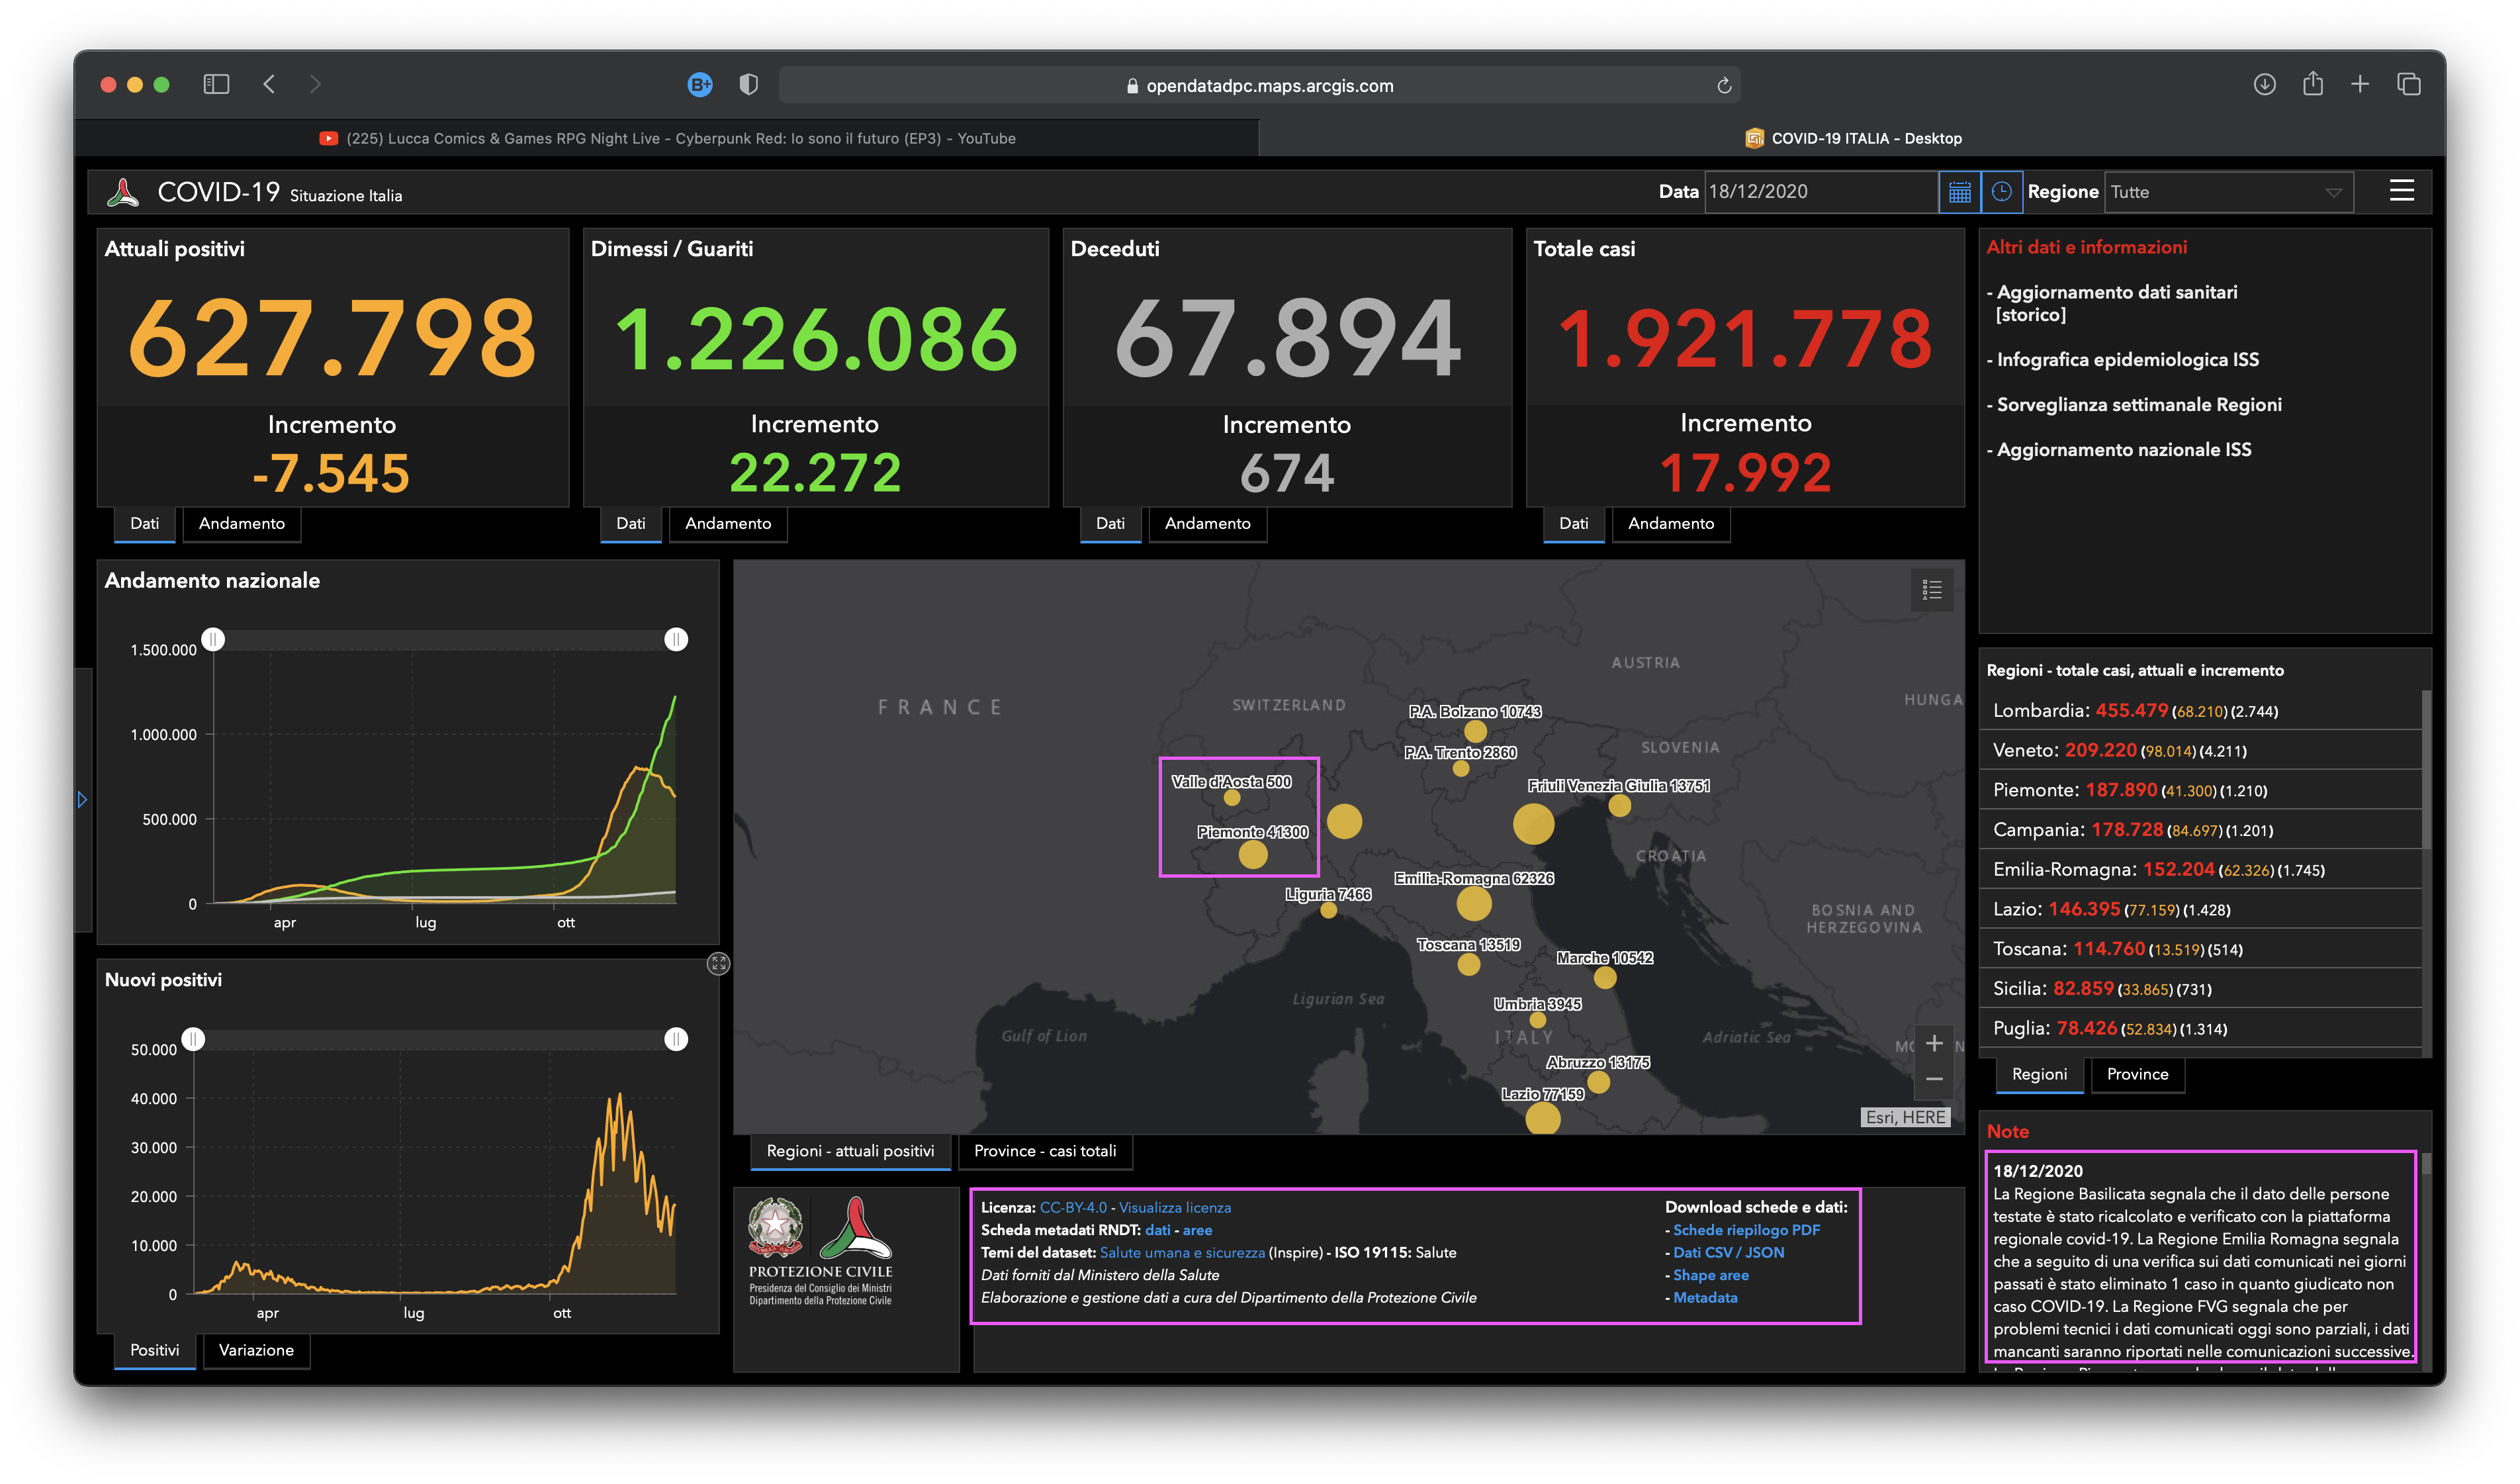
\includegraphics[width=0.5\columnwidth]{../../../assets/images/verifica-risorse-esistenti/guidelines_violations_1}
        \caption{Violazione della linea guida 1: testo troppo piccolo e quindi poco leggibile.}
        \label{fig:guidelines-violations-1}
    \end{figure}
    \item Limitazioni umane:
        \begin{enumerate}[label=\alph*.]
                \item Rispettata;
                \item Rispettata;
                \item [\ref{lg:2.c}] Violato nella sezione licenze;
                \item [d.] Rispettata;
                \item [\ref{lg:2.e}] Violato nella sidebar in cui è illustrata la dashboard e come mostrato nel rettangolo viola in ~\ref{fig:guidelines-violations-2}.
                \begin{figure}[H]
                    \centering
                    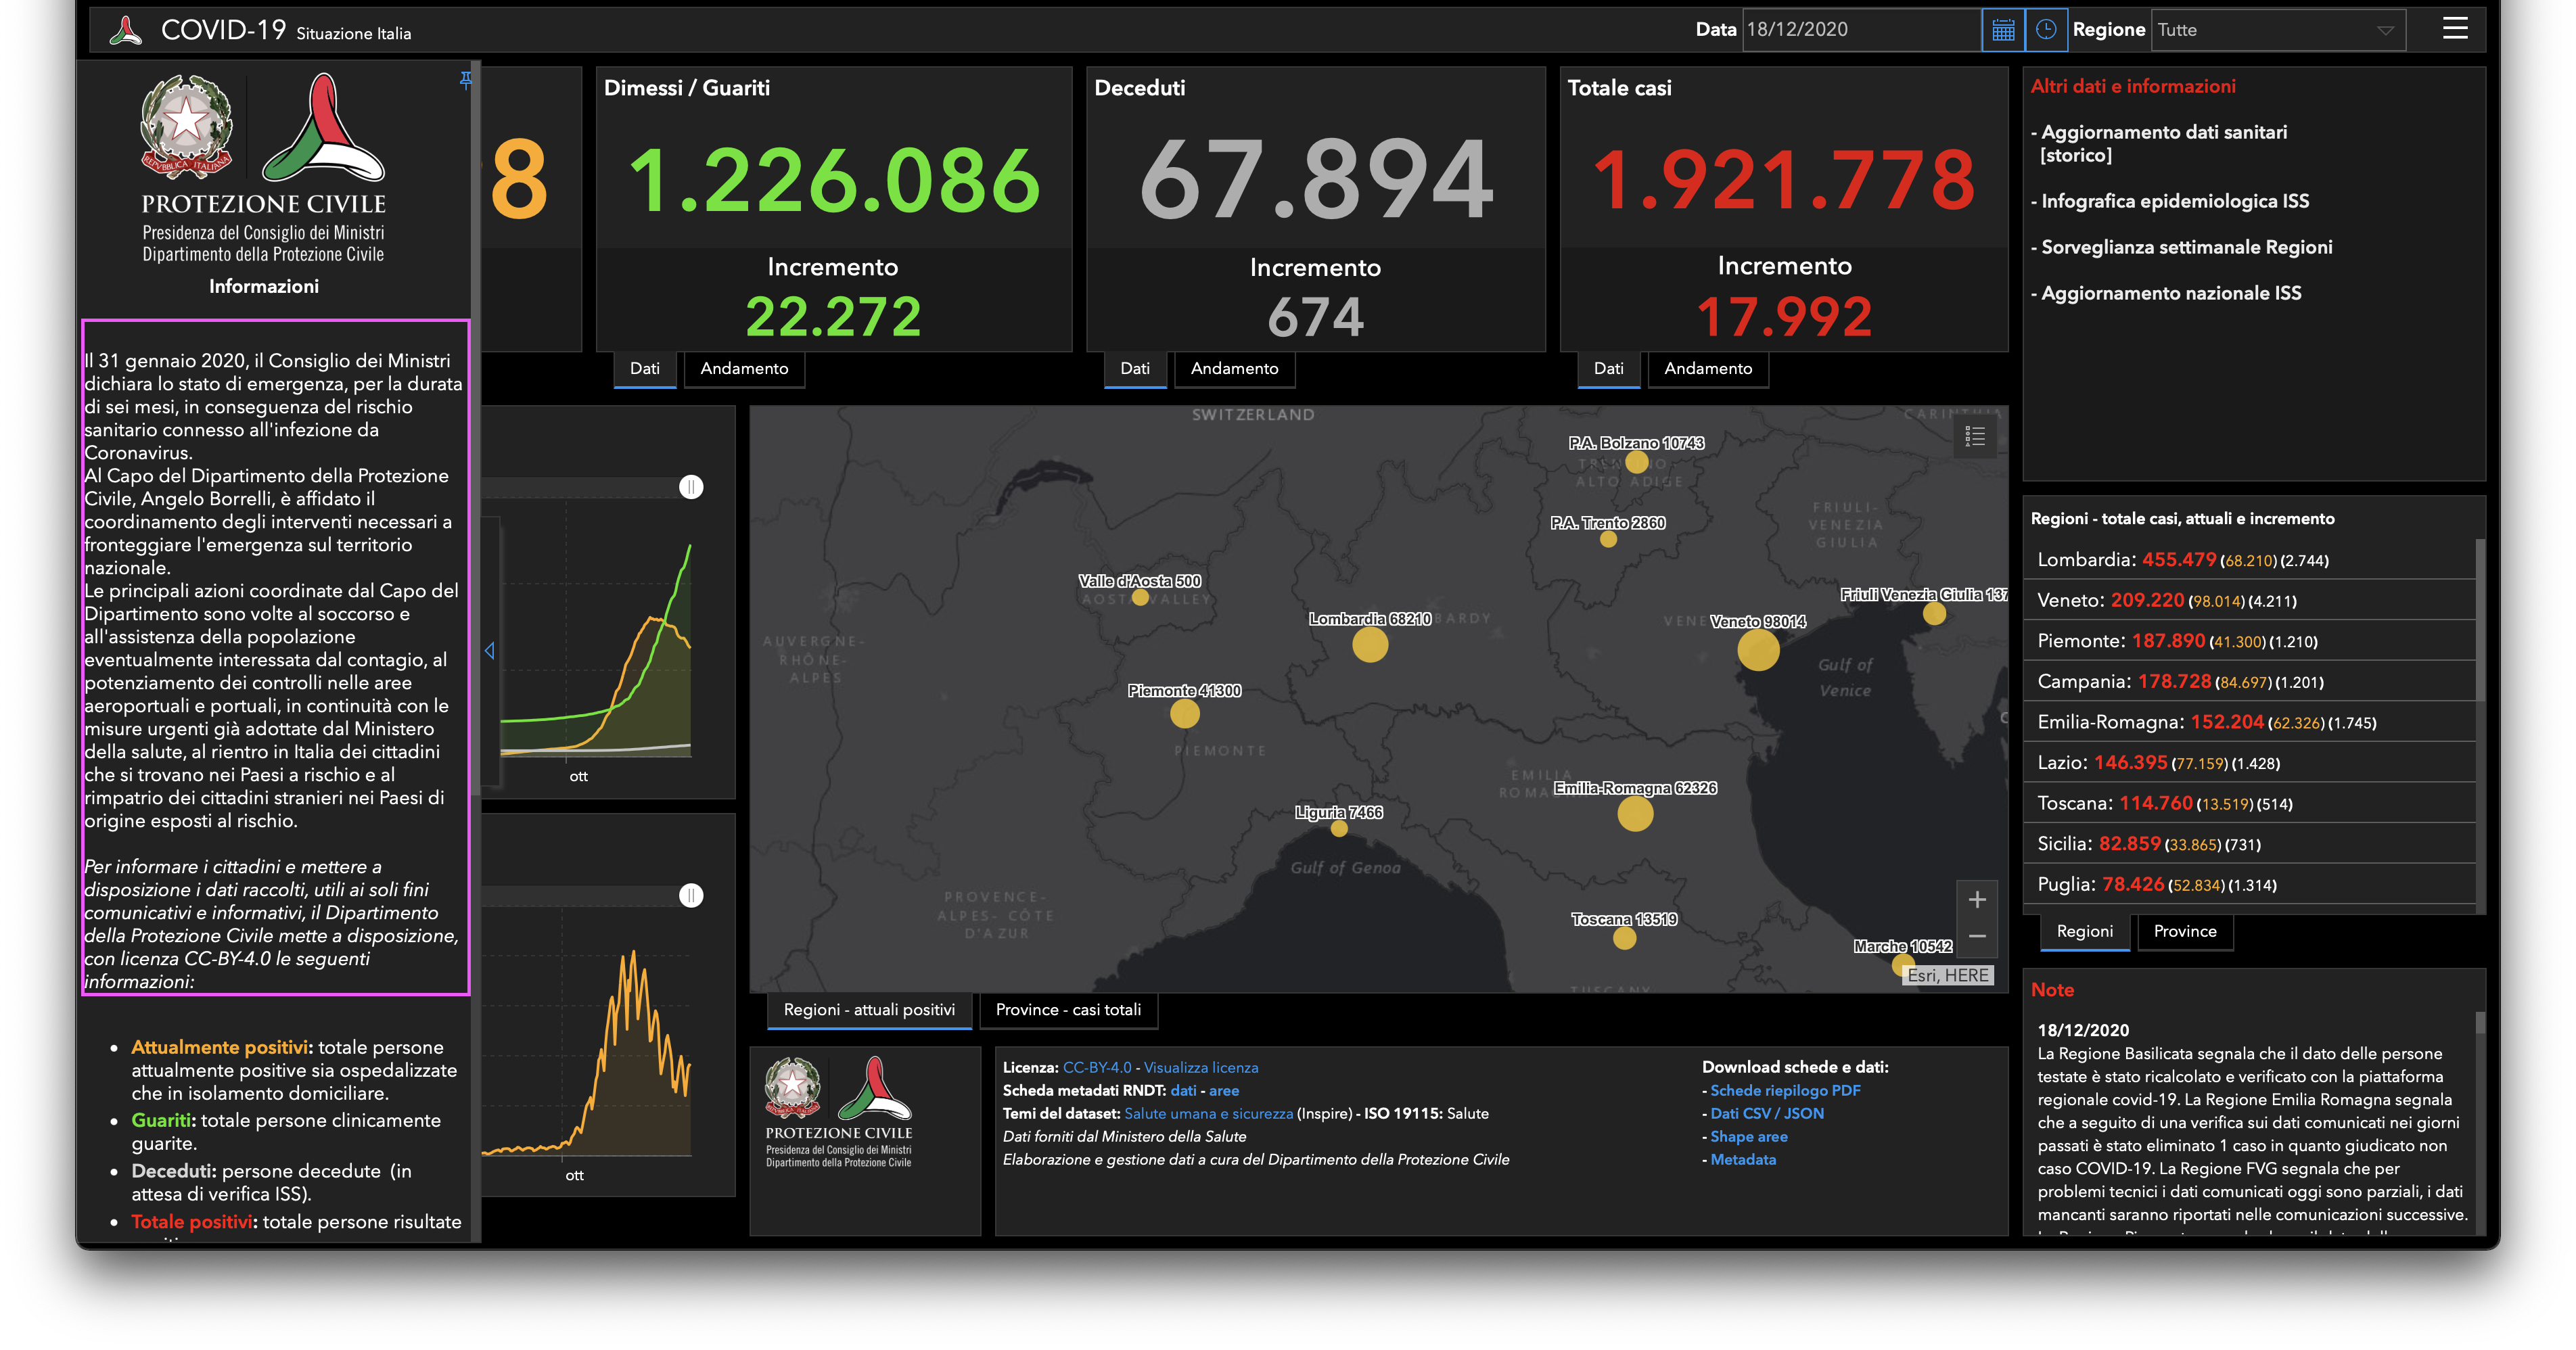
\includegraphics[width=0.5\columnwidth]{../../../assets/images/verifica-risorse-esistenti/guidelines_violations_2}
                    \caption{Violazione della linea guida 2.e: le linee contengono meno di cinquanta caratteri.}
                    \label{fig:guidelines-violations-2}
                \end{figure}
        \end{enumerate}
    \item I valori numerici non sono organizzati in blocchi non permettendo un agevole confronto come mostrato in ~\ref{fig:guidelines-violations-3}. Inoltre nel modal evidenziato in viola in ~\ref{fig:guidelines-violations-4} che rappresenta i dati di una regione c'è solo un elencon senza struttura con etichette difficilmente leggibili in quanto scritte con gli underscore al posto degli spazi;
        \begin{figure}[H]
            \centering
            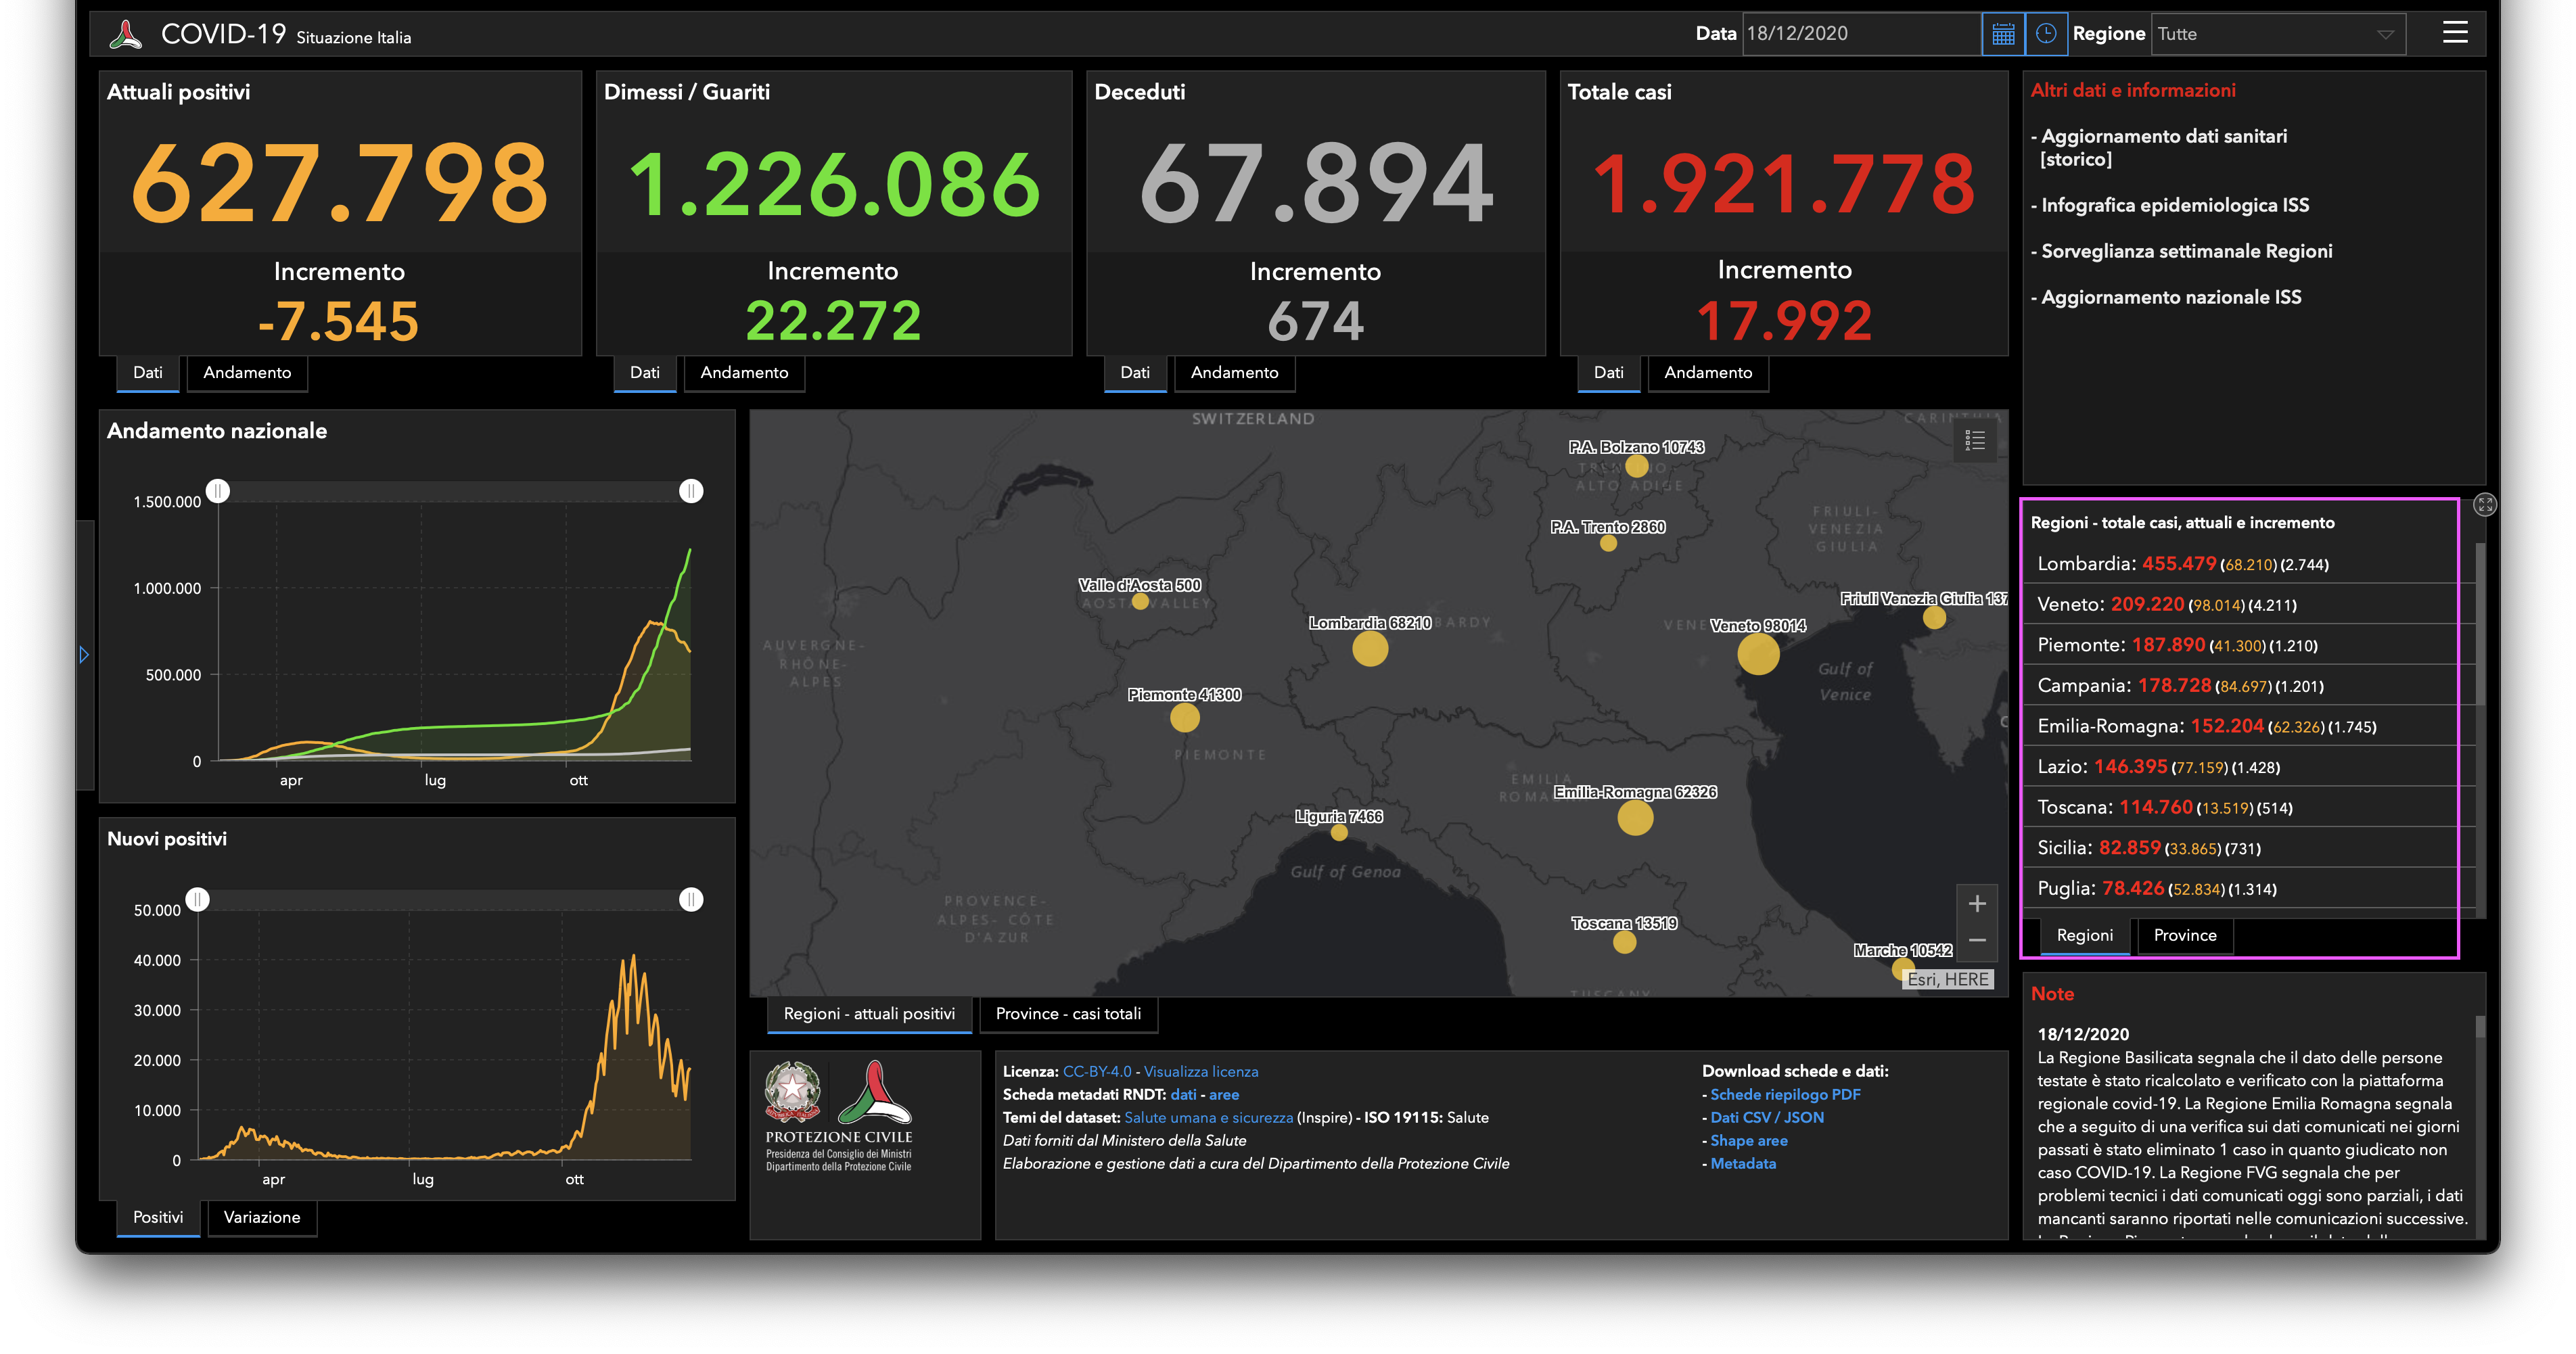
\includegraphics[width=0.5\columnwidth]{../../../assets/images/verifica-risorse-esistenti/guidelines_violations_3}
            \caption{Violazione della linea guida 3: I numeri non sono raggrupati.}
            \label{fig:guidelines-violations-3}
        \end{figure}
        \begin{figure}[H]
            \centering
            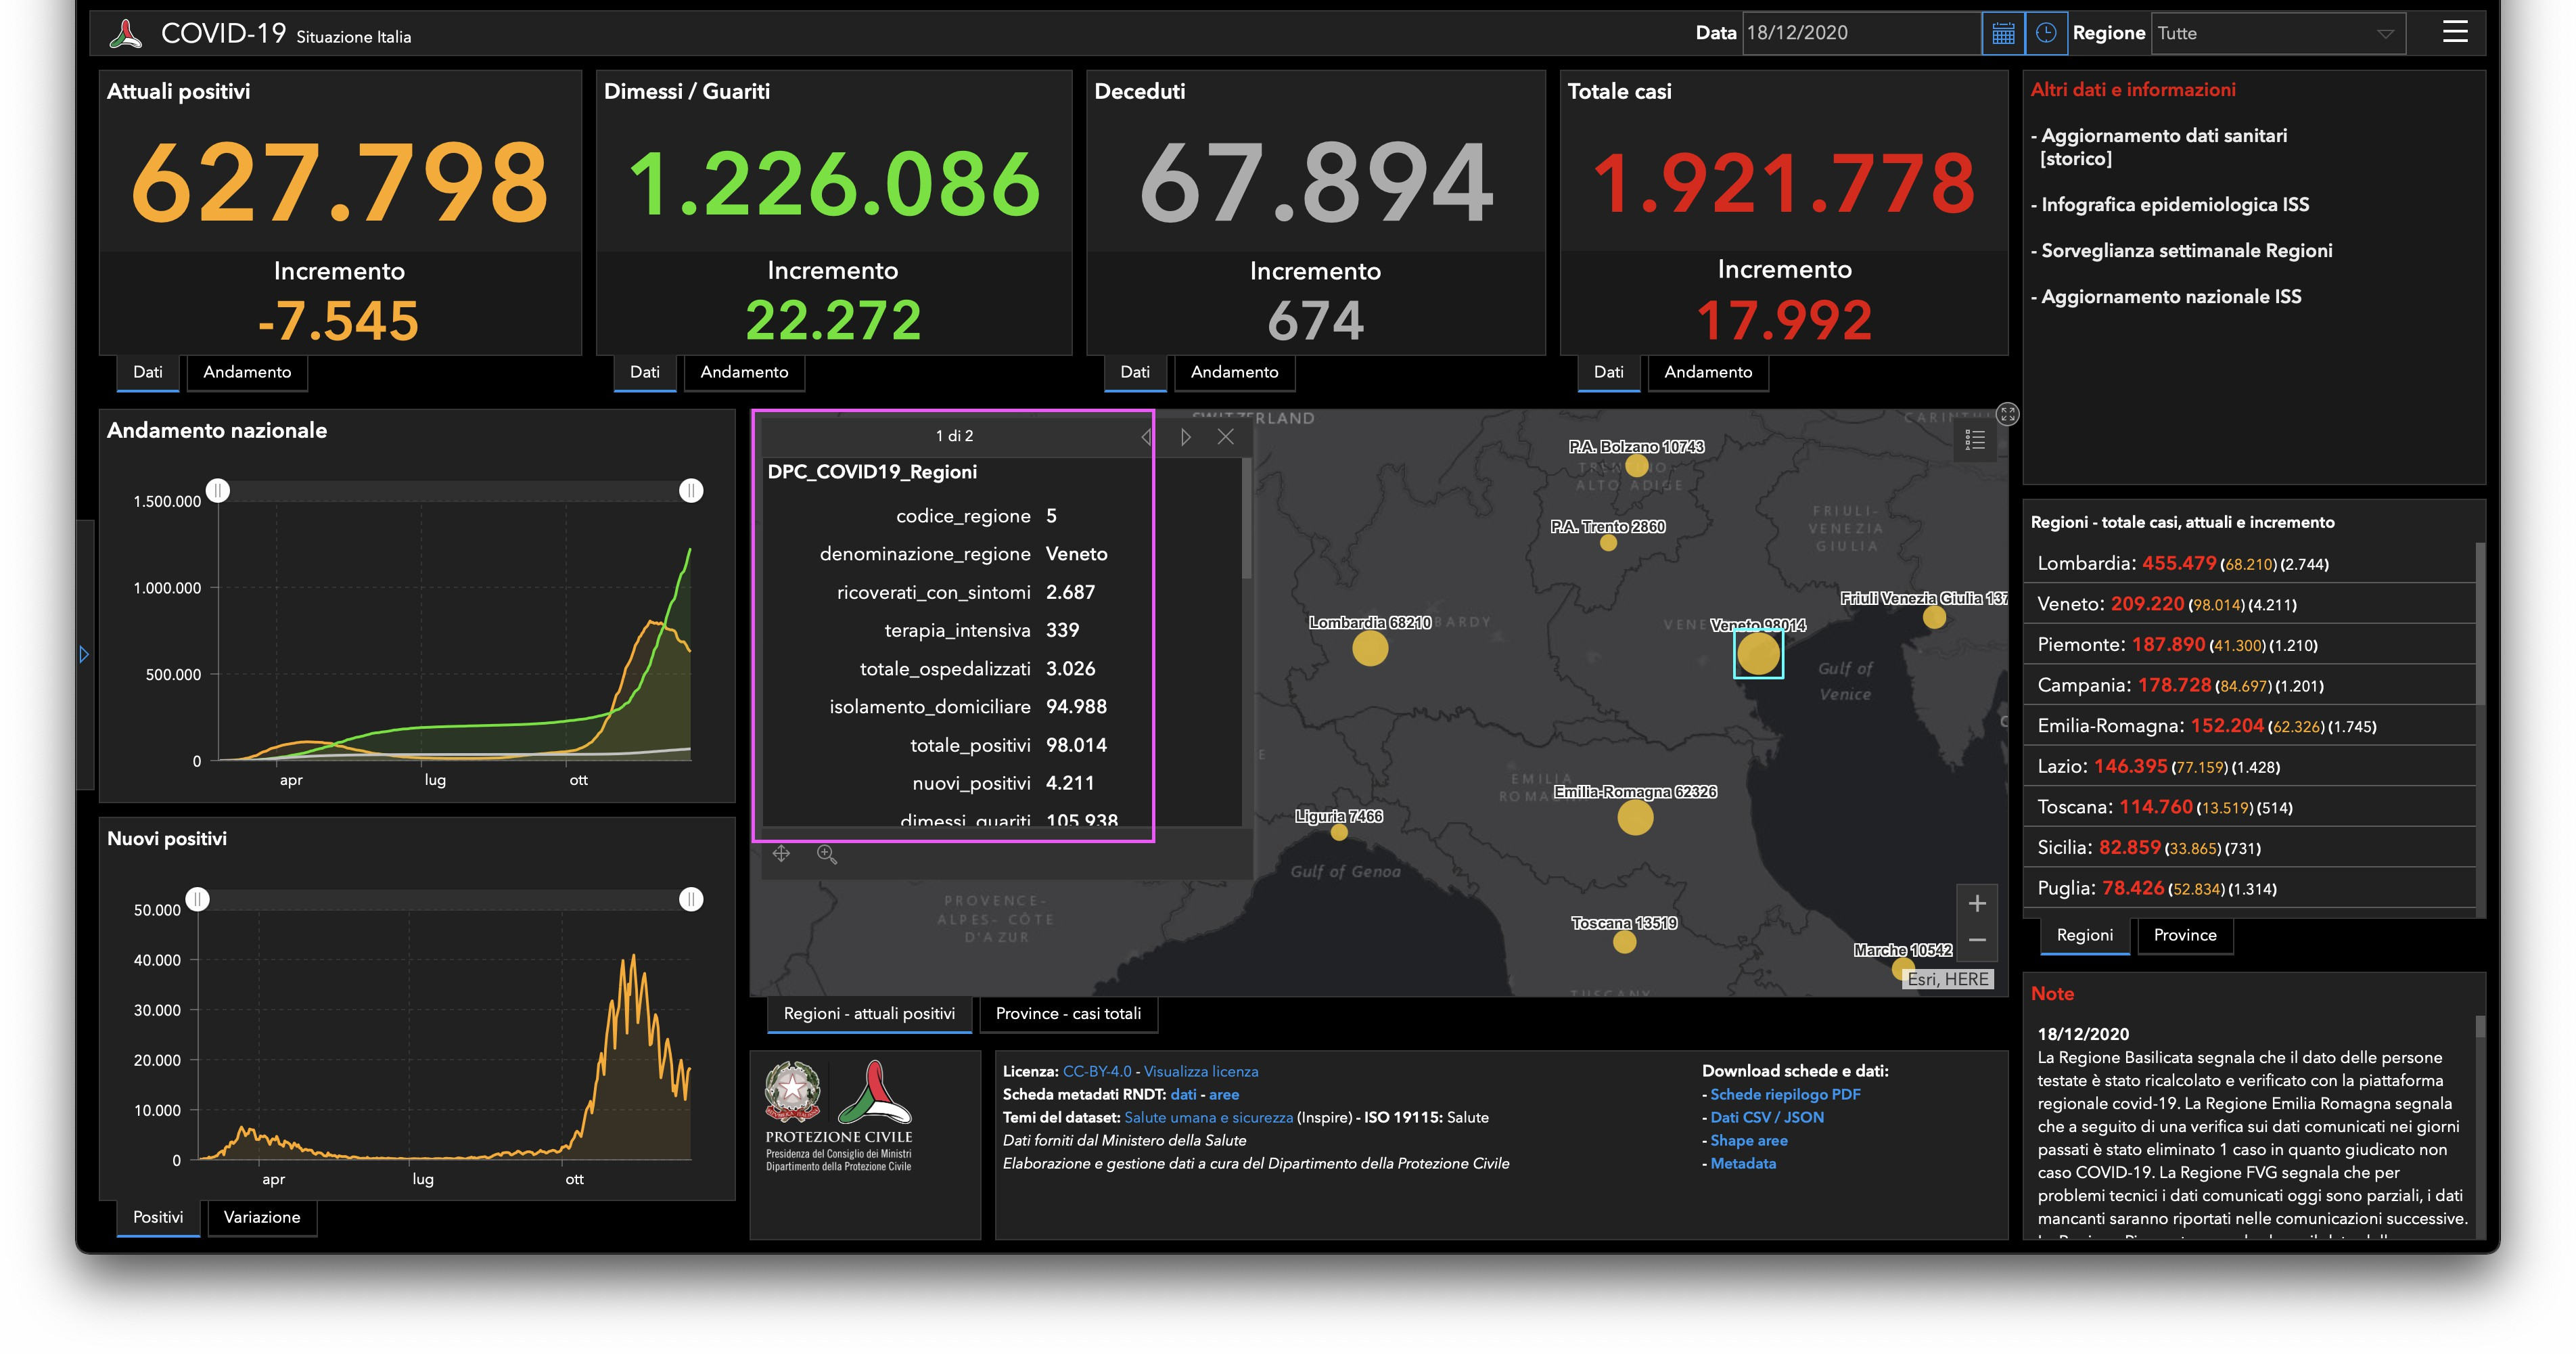
\includegraphics[width=0.5\columnwidth]{../../../assets/images/verifica-risorse-esistenti/guidelines_violations_4}
            \caption{Violazione della linea guida 3: I valori e i numeri sono difficilmente comprensibili.}
            \label{fig:guidelines-violations-4}
        \end{figure}
    \item Rispettata; 
    \item La memoria funziona meglio riconoscendo gli oggetti:
        \begin{enumerate}[label=\alph*.]
            \item Rispettata;
            \item [\ref{lg:5.b}] Il percorso di lettura non è ottimale: i primi quattro riquadri vanno bene ma, il resto, da come si nota in ~\ref{fig:guidelines-violations-5} non è molto chiaro.
                \begin{figure}[H]
                    \centering
                    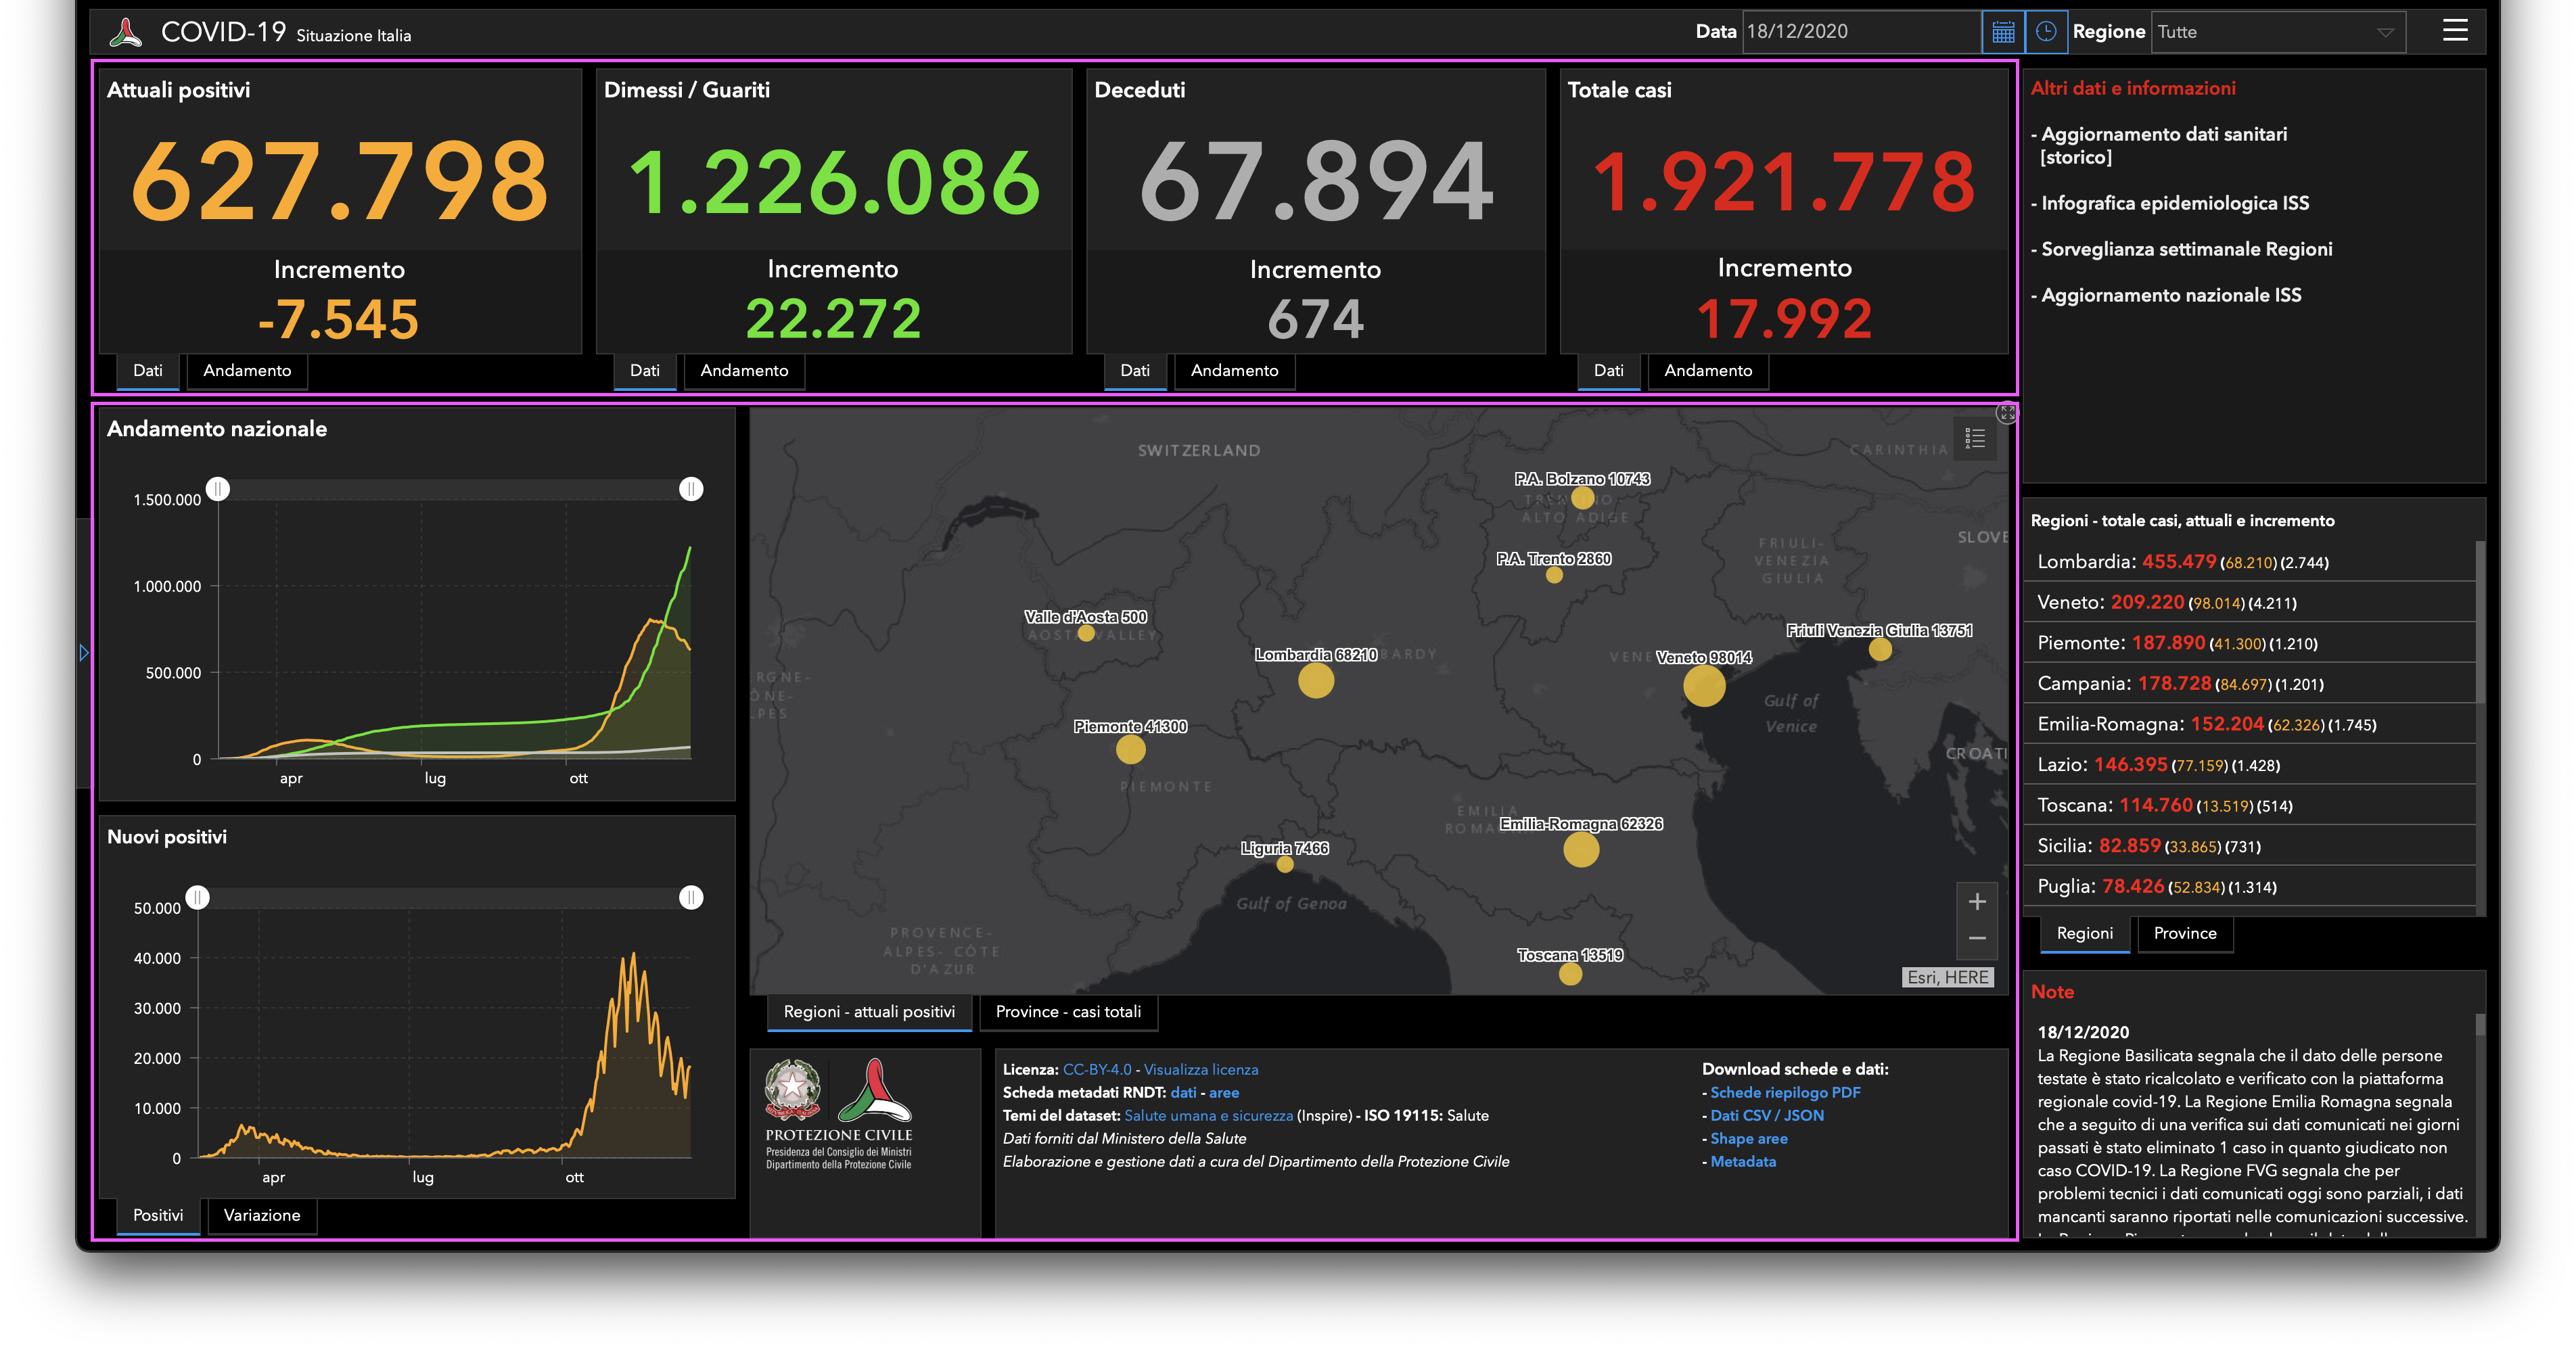
\includegraphics[width=0.5\columnwidth]{../../../assets/images/verifica-risorse-esistenti/guidelines_violations_5}
                    \caption{Violazione della linea guida 5.b: il percorso di lettura non è ottimale.}
                    \label{fig:guidelines-violations-5}
                \end{figure}
        \end{enumerate}
    \item Rispettata;
    \item Rispettata;
    \item La funzionalità evidenziata in ~\ref{fig:guidelines-violations-6} permette di cambiare la visualizzazione della pagina, ma risulta poco visibile e non è ben segnalato;
    \item Rispettata;
        \begin{figure}[H]
            \centering
            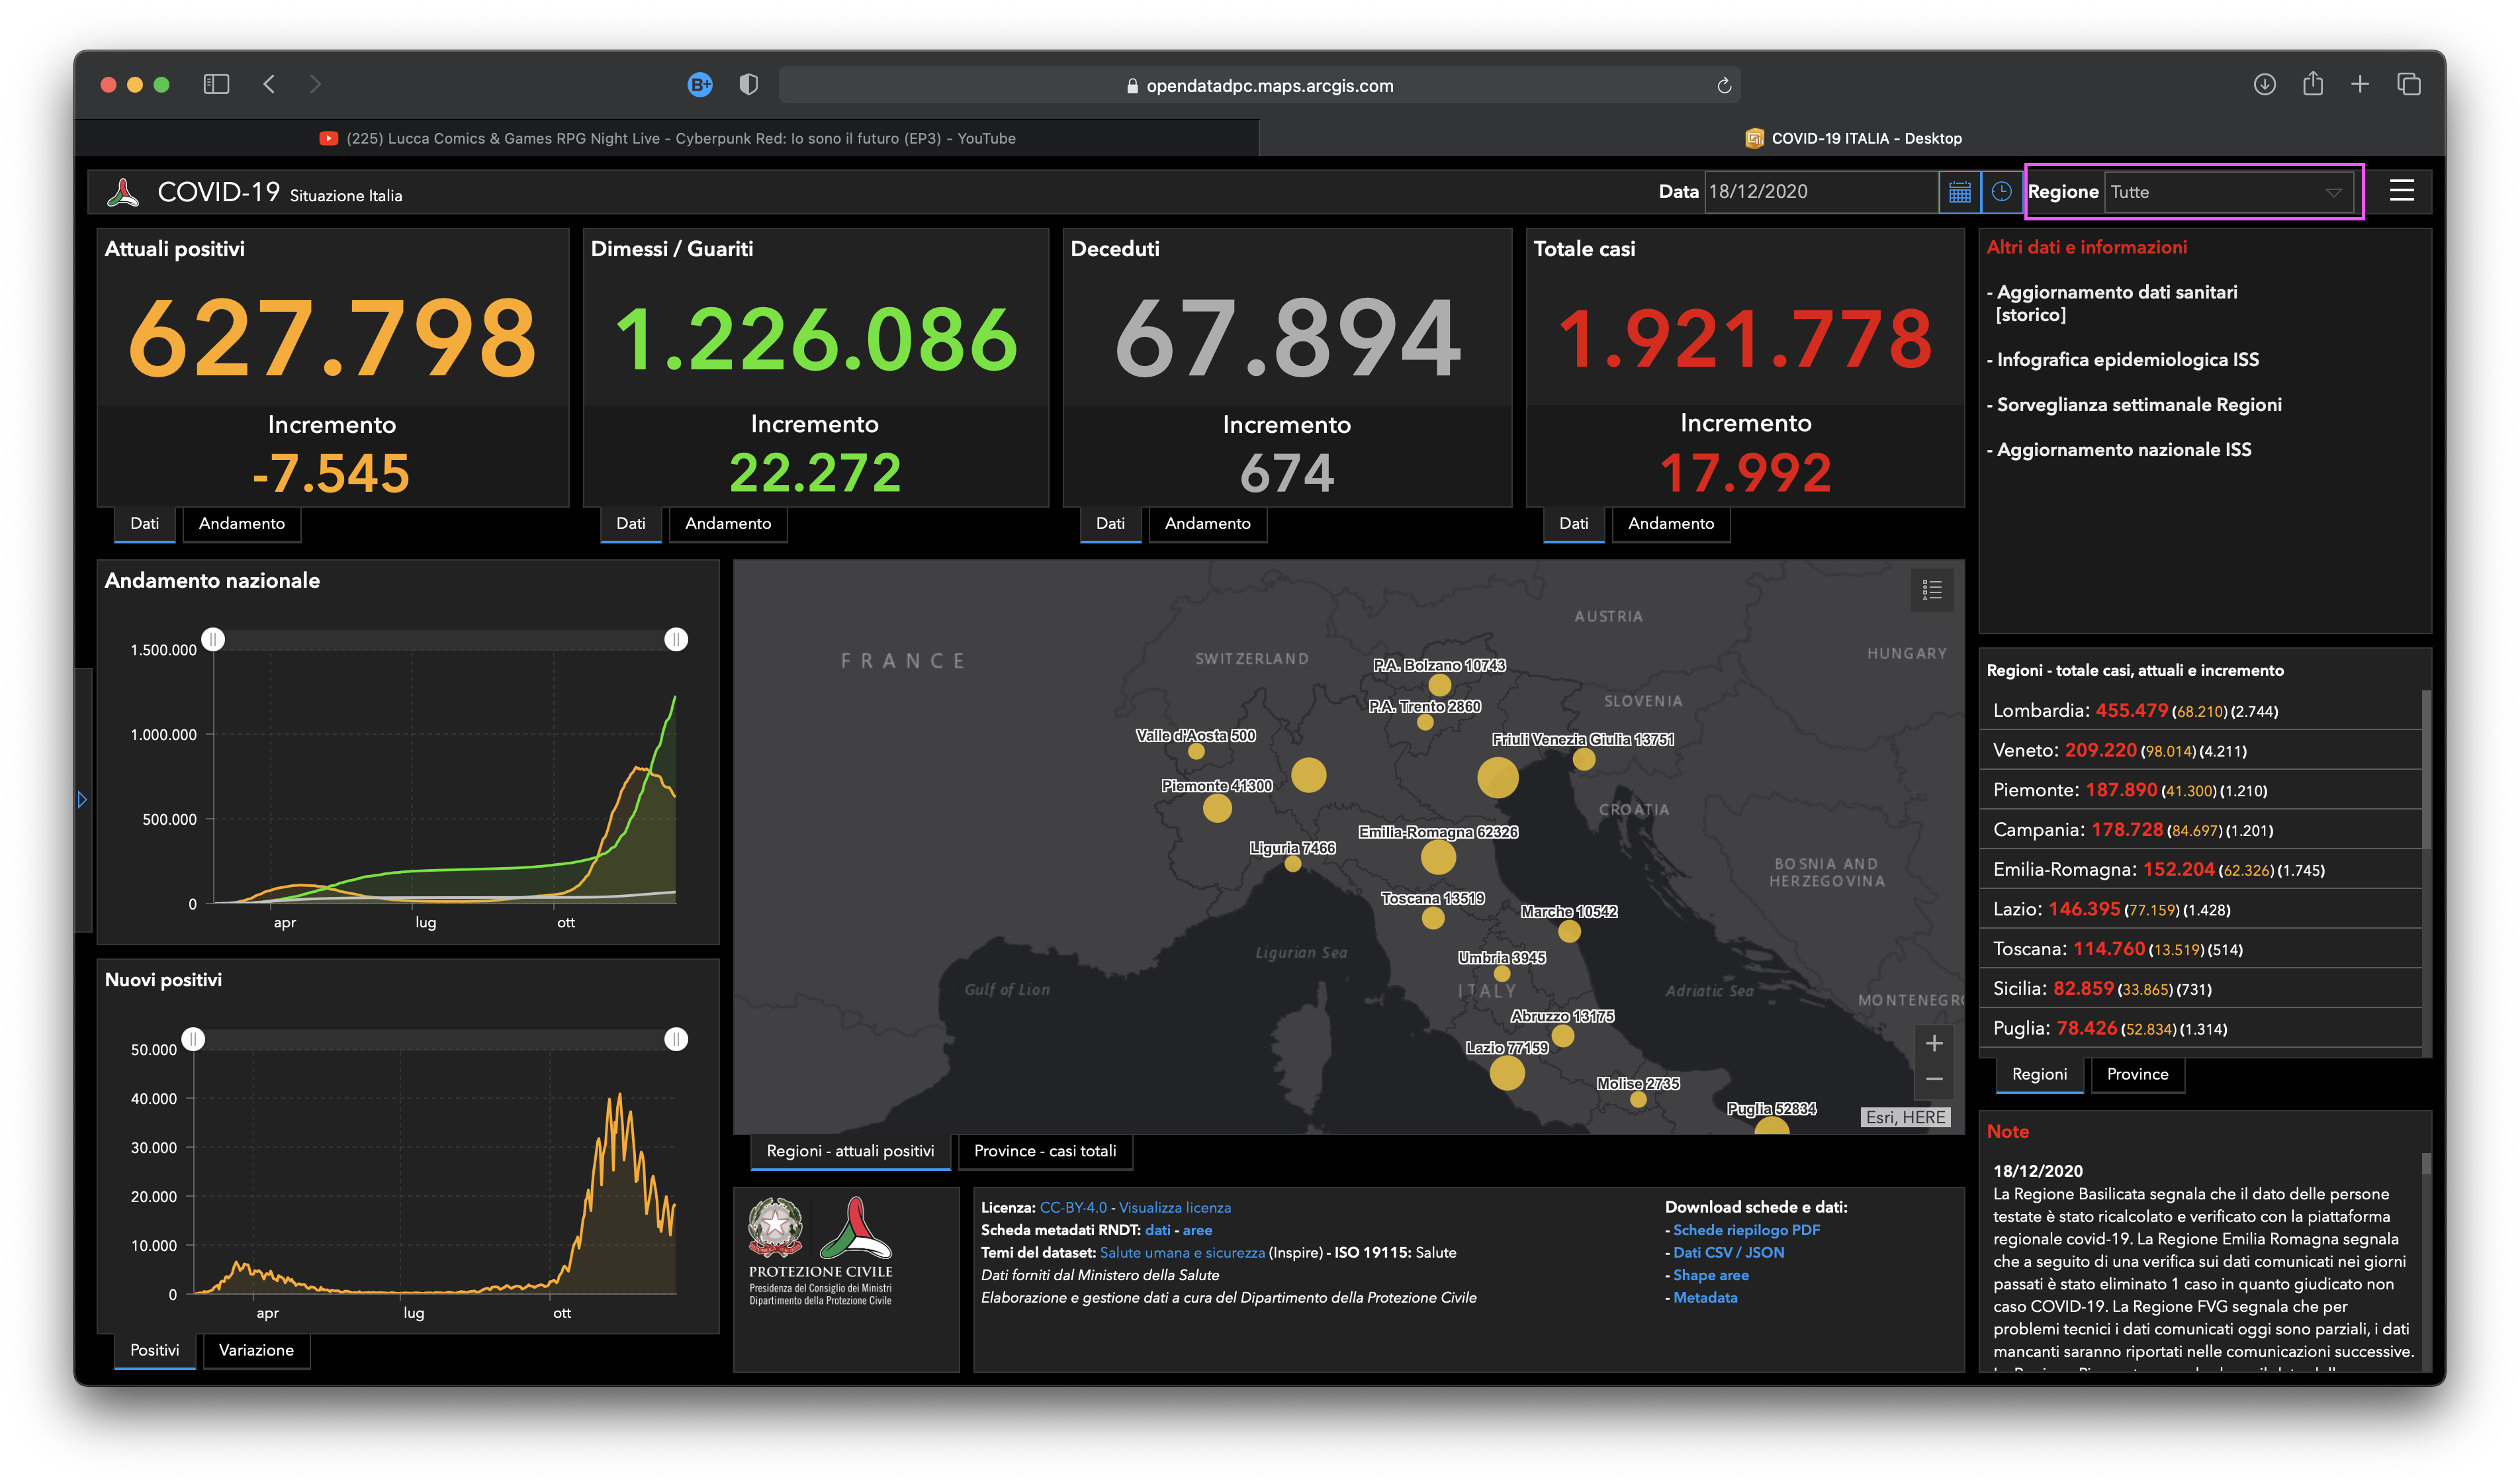
\includegraphics[width=0.5\columnwidth]{../../../assets/images/verifica-risorse-esistenti/guidelines_violations_6}
            \caption{Violazione della linea guida 5.b: il percorso di lettura non è ottimale.}
            \label{fig:guidelines-violations-6}
        \end{figure}
    \item Varie analisi (task) sono particolarmente scomode per essere realizzate (situazione terapie intensive);
    \item Non vi sono indicazioni su come la dashboard possa essere utilizzata;
    \item Rispettata;
    \item Rispettata;
    \item Sono presenti solamente valori assoluti (cumulativi e variazioni);
    \item Rispettata;
    \item Rispettata;
    \item Una persona affetta da daltonismo nota che i primi due blocchi (attuali positivi e dimessi/guariti) sono poco riconoscibili in quanto i colori si assomigliano;
    \item Rispettata;
    \item Validità del contenuto:
        \begin{enumerate}[label=\alph*.]
            \item [\ref{lg:19.a}] Non è presente la data dell'ultimo aggiornamento;
            \item [b.] Rispettata;
        \end{enumerate}
    \item Rispettate;
    \item Rispettata;
    \item Non sono presenti contatti o form di contatto;
    \item Rispettata;
    \item Rispettata;
    \item Zoom-in e Zoom-out non sono funzionalità sufficienti in una mappa: ad esempio, se per errore o per intenzione ci si sposta troppo dal centro della mappa è bene avere un pulsante di reset;
        \begin{figure}[H]
            \centering
            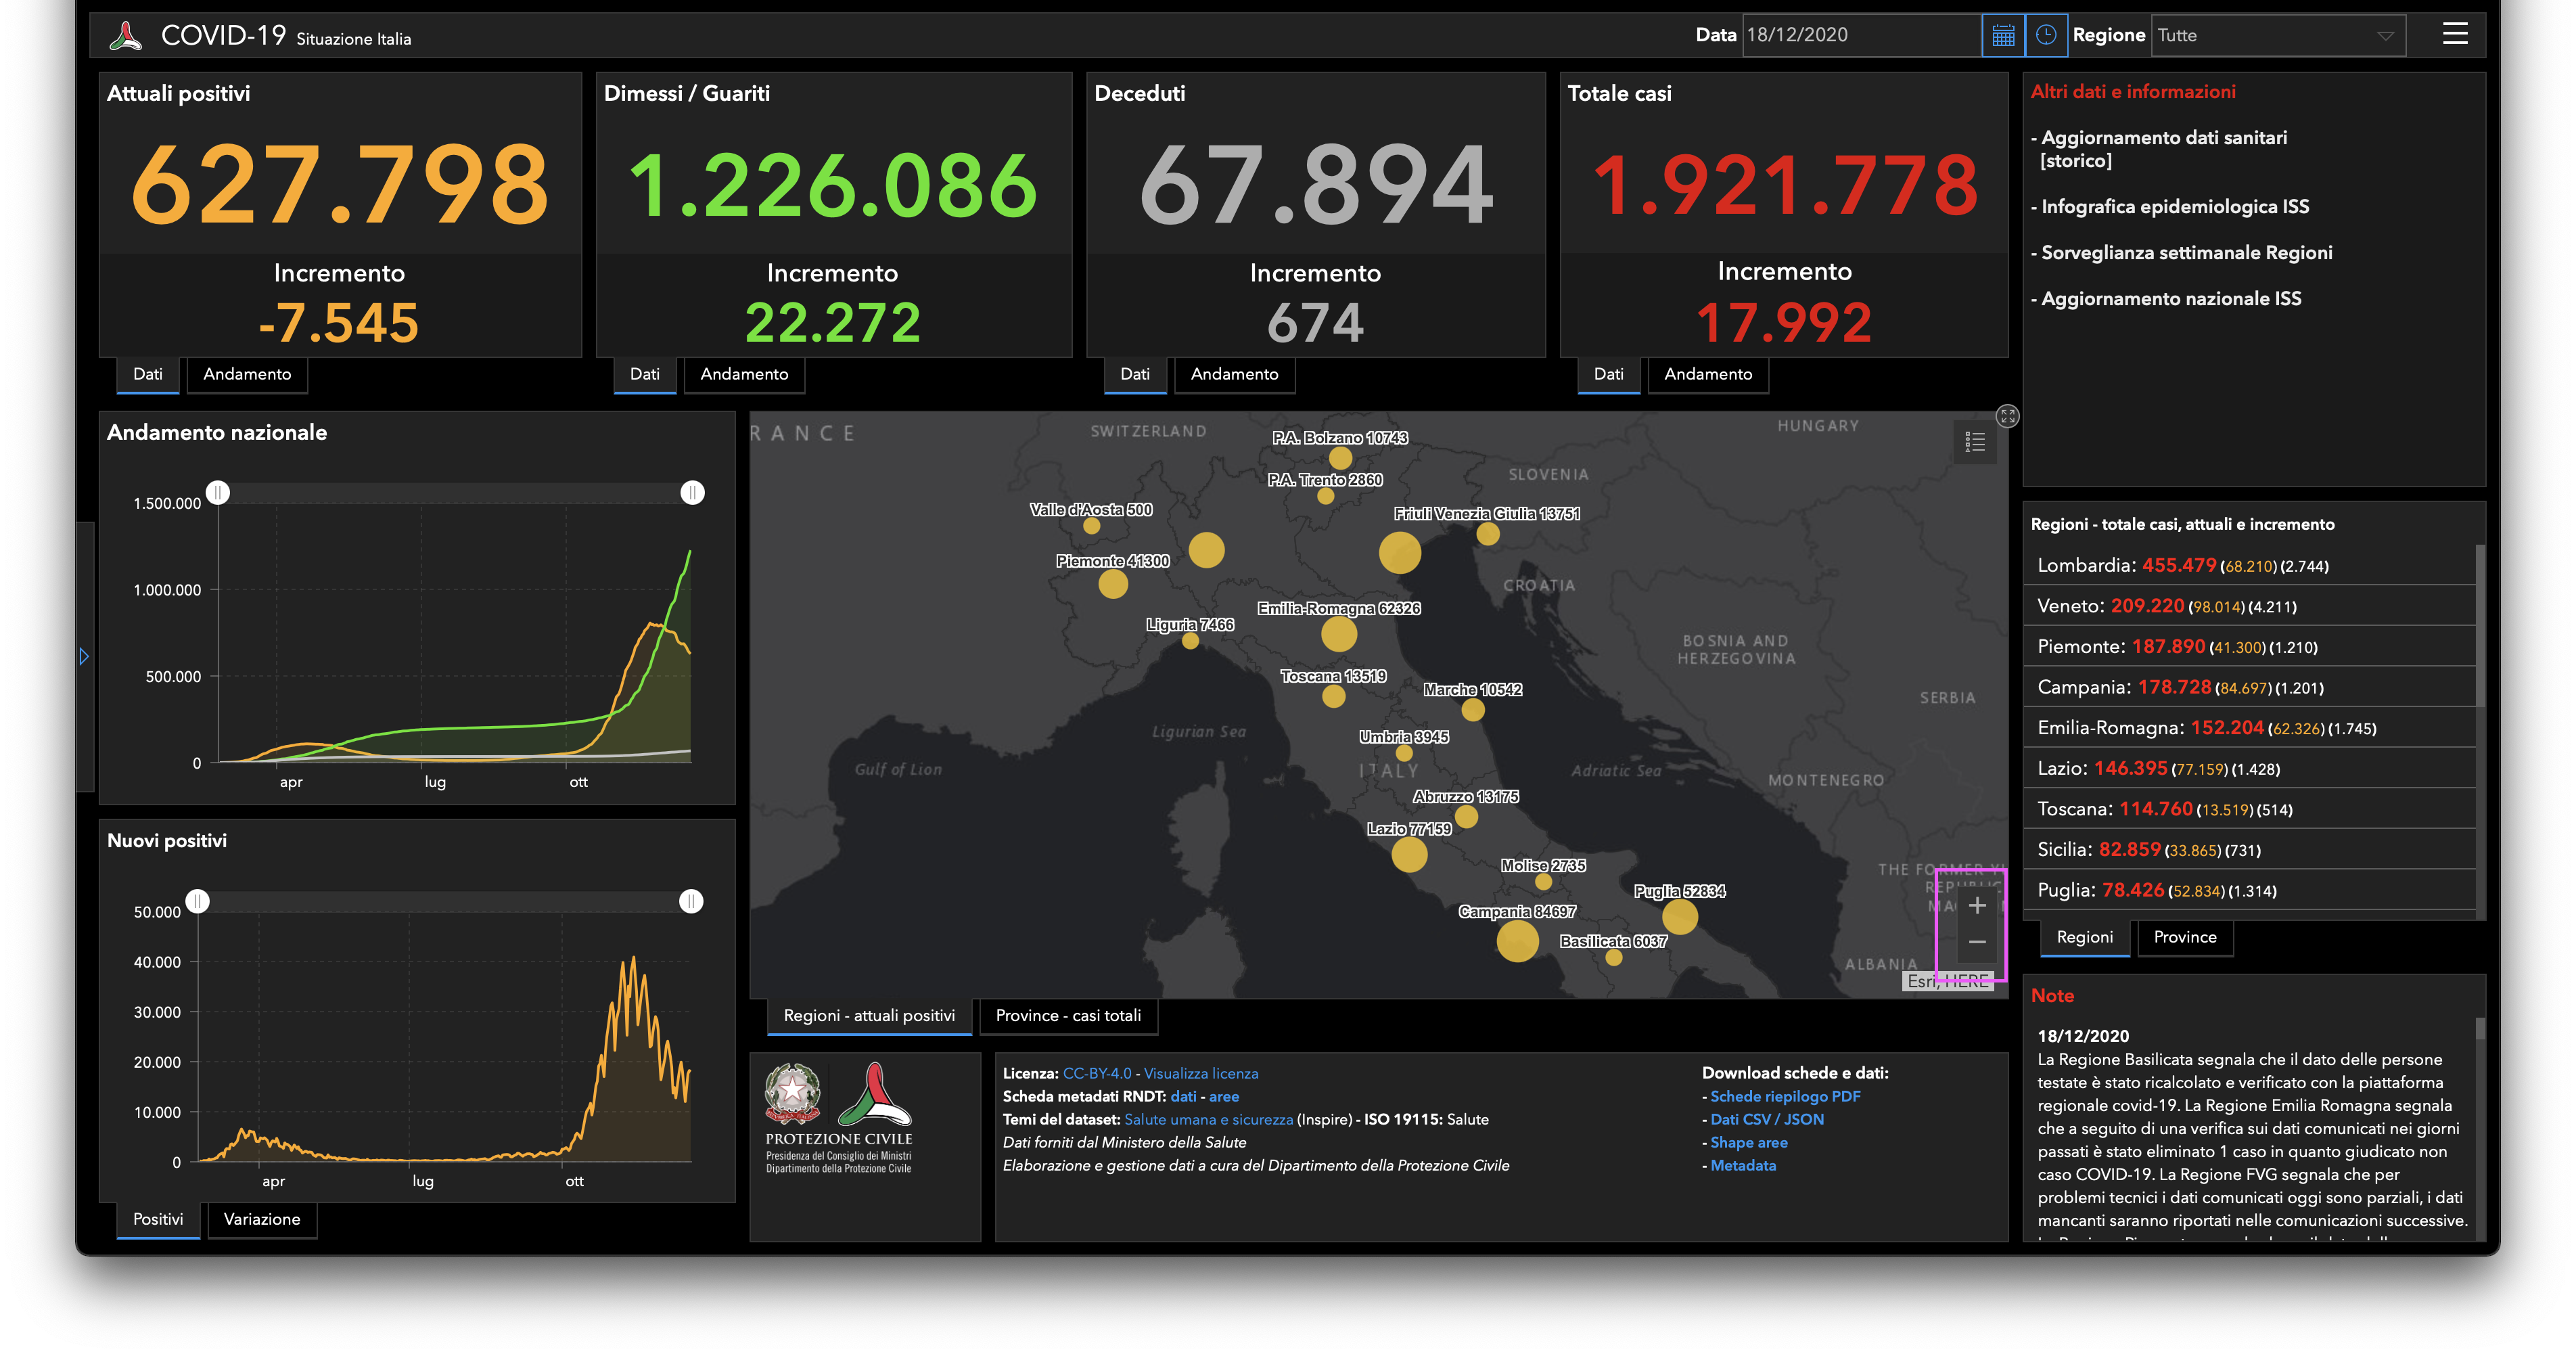
\includegraphics[width=0.5\columnwidth]{../../../assets/images/verifica-risorse-esistenti/guidelines_violations_7}
            \caption{Violazione della linea guida 25: funzionalità non sufficienti sulla mappa.}
            \label{fig:guidelines-violations-7}
        \end{figure}
    \item Assenza di meccanismi di prevenzione degli errori:
        \begin{enumerate}[label=\alph*.]
            \item [\ref{lg:26.a}] In ~\ref{fig:guidelines-violations-8} si nota come si possono selezionare date future mentre in ~\ref{fig:guidelines-violations-9} come sia possibile scrivere un qualsiasi testo al posto della data;

            \begin{figure}[H]
                \centering
                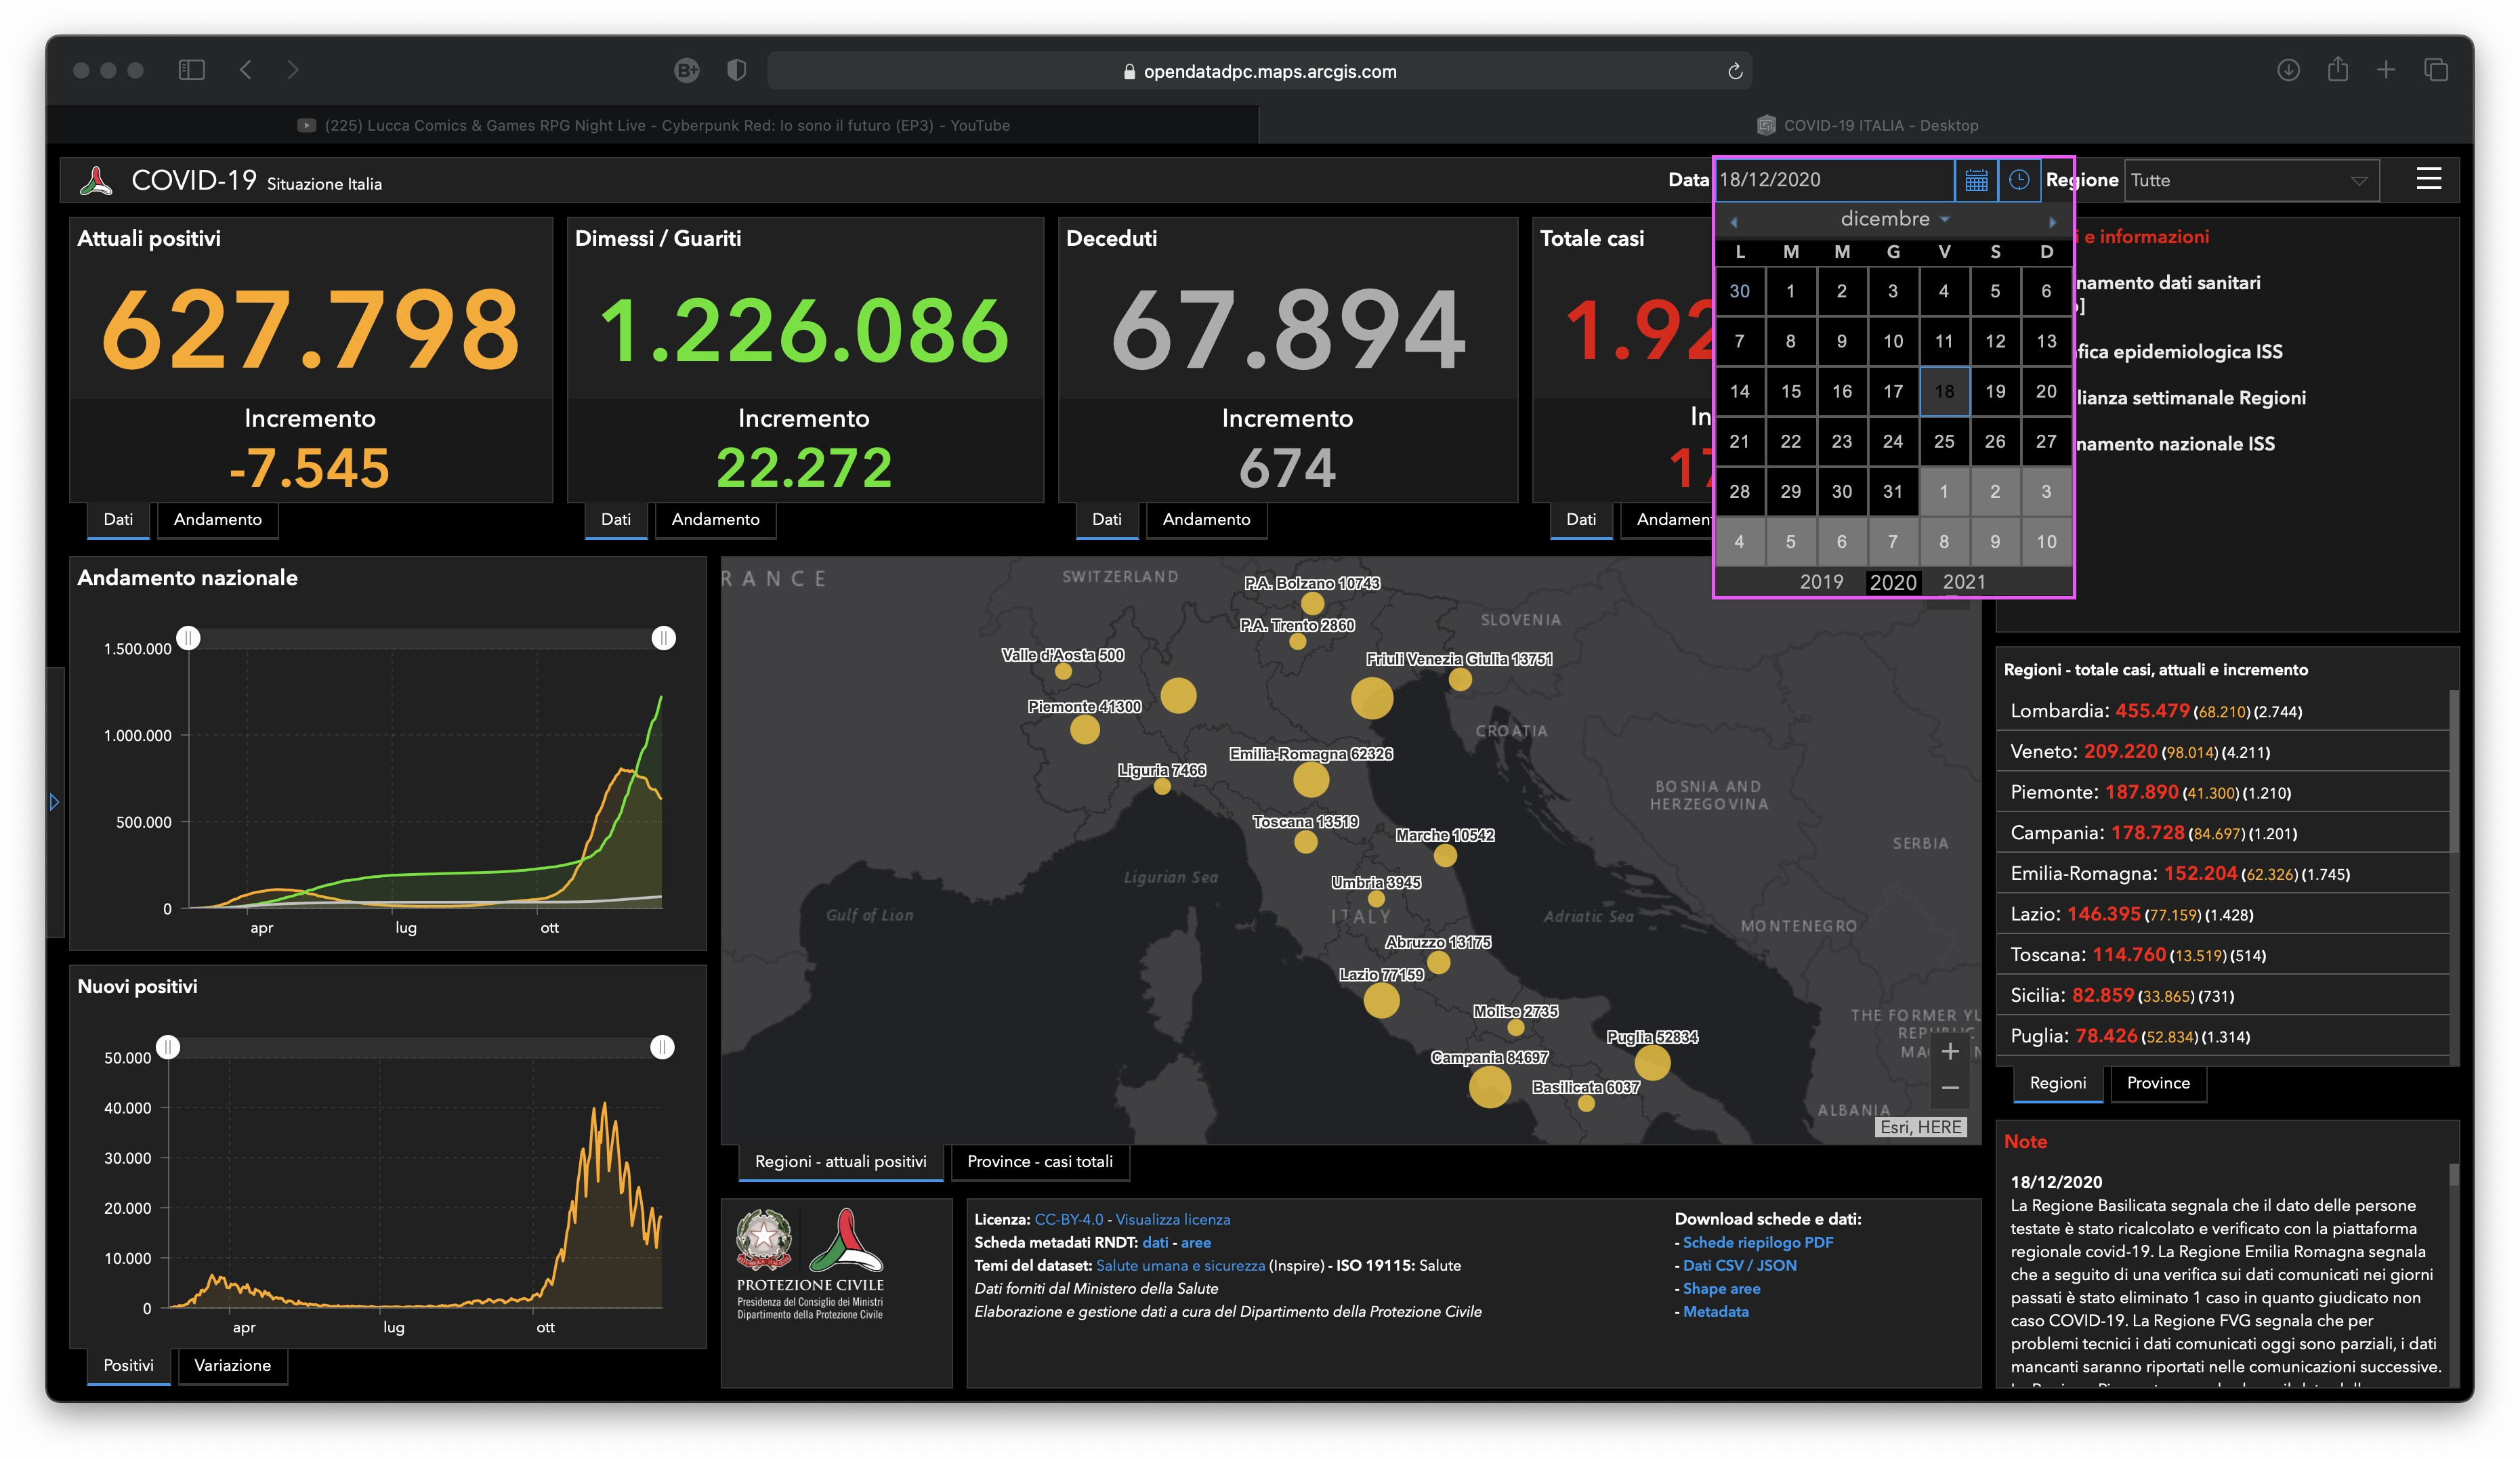
\includegraphics[width=0.5\columnwidth]{../../../assets/images/verifica-risorse-esistenti/guidelines_violations_8}
                \caption{Violazione della linea guida 26.a: date future selezionabili.}
                \label{fig:guidelines-violations-8}
            \end{figure}
            \begin{figure}[H]
                \centering
                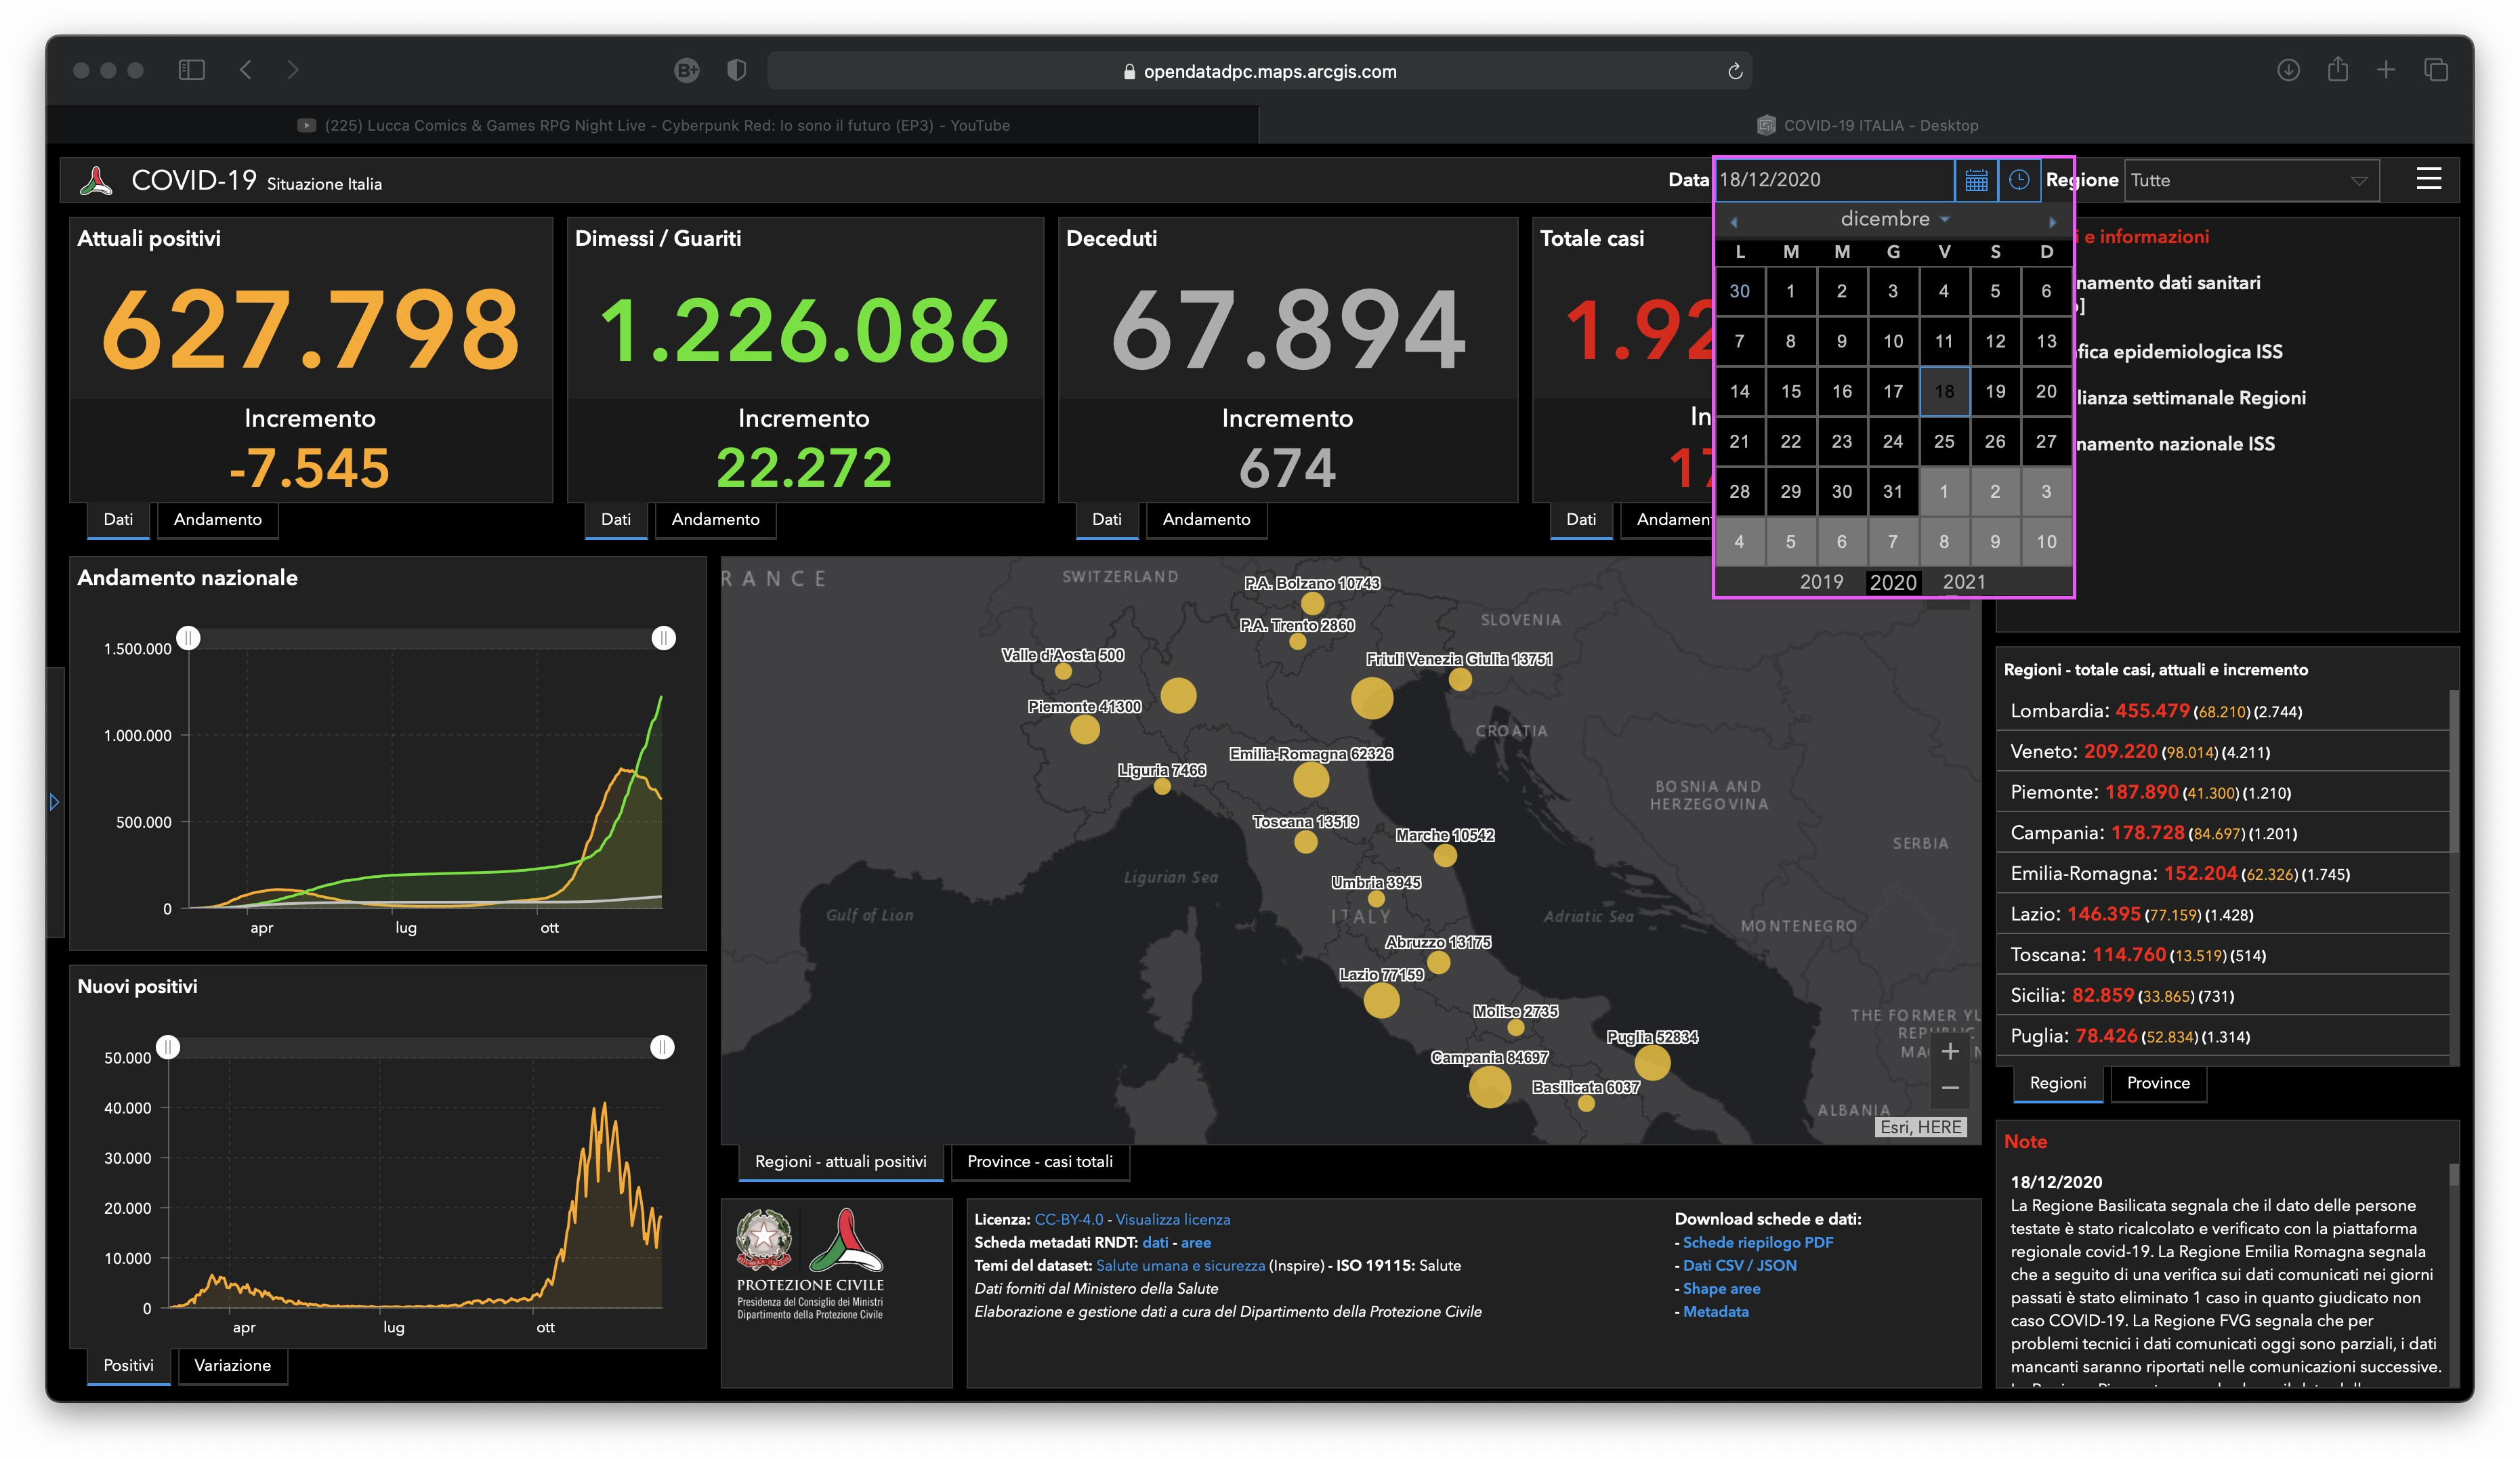
\includegraphics[width=0.5\columnwidth]{../../../assets/images/verifica-risorse-esistenti/guidelines_violations_8}
                \caption{Violazione della linea guida 26.b: casella di testo che accetta qualsiasi input.}
                \label{fig:guidelines-violations-9}
            \end{figure}
        \end{enumerate}
    \item Flessibilità ed efficienza all'uso:
        \begin{enumerate}[label=\alph*.]
            \item [\ref{lg:27.a}] Un utente ``PRO" non ha modo di salvare le sue preferenze/modalità di visualizzazione;
            \item [\ref{lg:27.b}] Non ci sono shortcut utilizzabili.
        \end{enumerate}
    \item Non ci sono spiegazioni su come usare il sistema;
    \item Il sistema non è prevedibile: se si clicca sul nome di una regione oppure se sulla mappa si zoomma su di una regione ci si aspetta di visualizzare le province con i rispettivi valori e invece ciò non accade come mostrato in ~\ref{fig:guidelines-violations-10};
        \begin{figure}[H]
            \centering
            \begin{subfigure}[b]{0.5\columnwidth}
                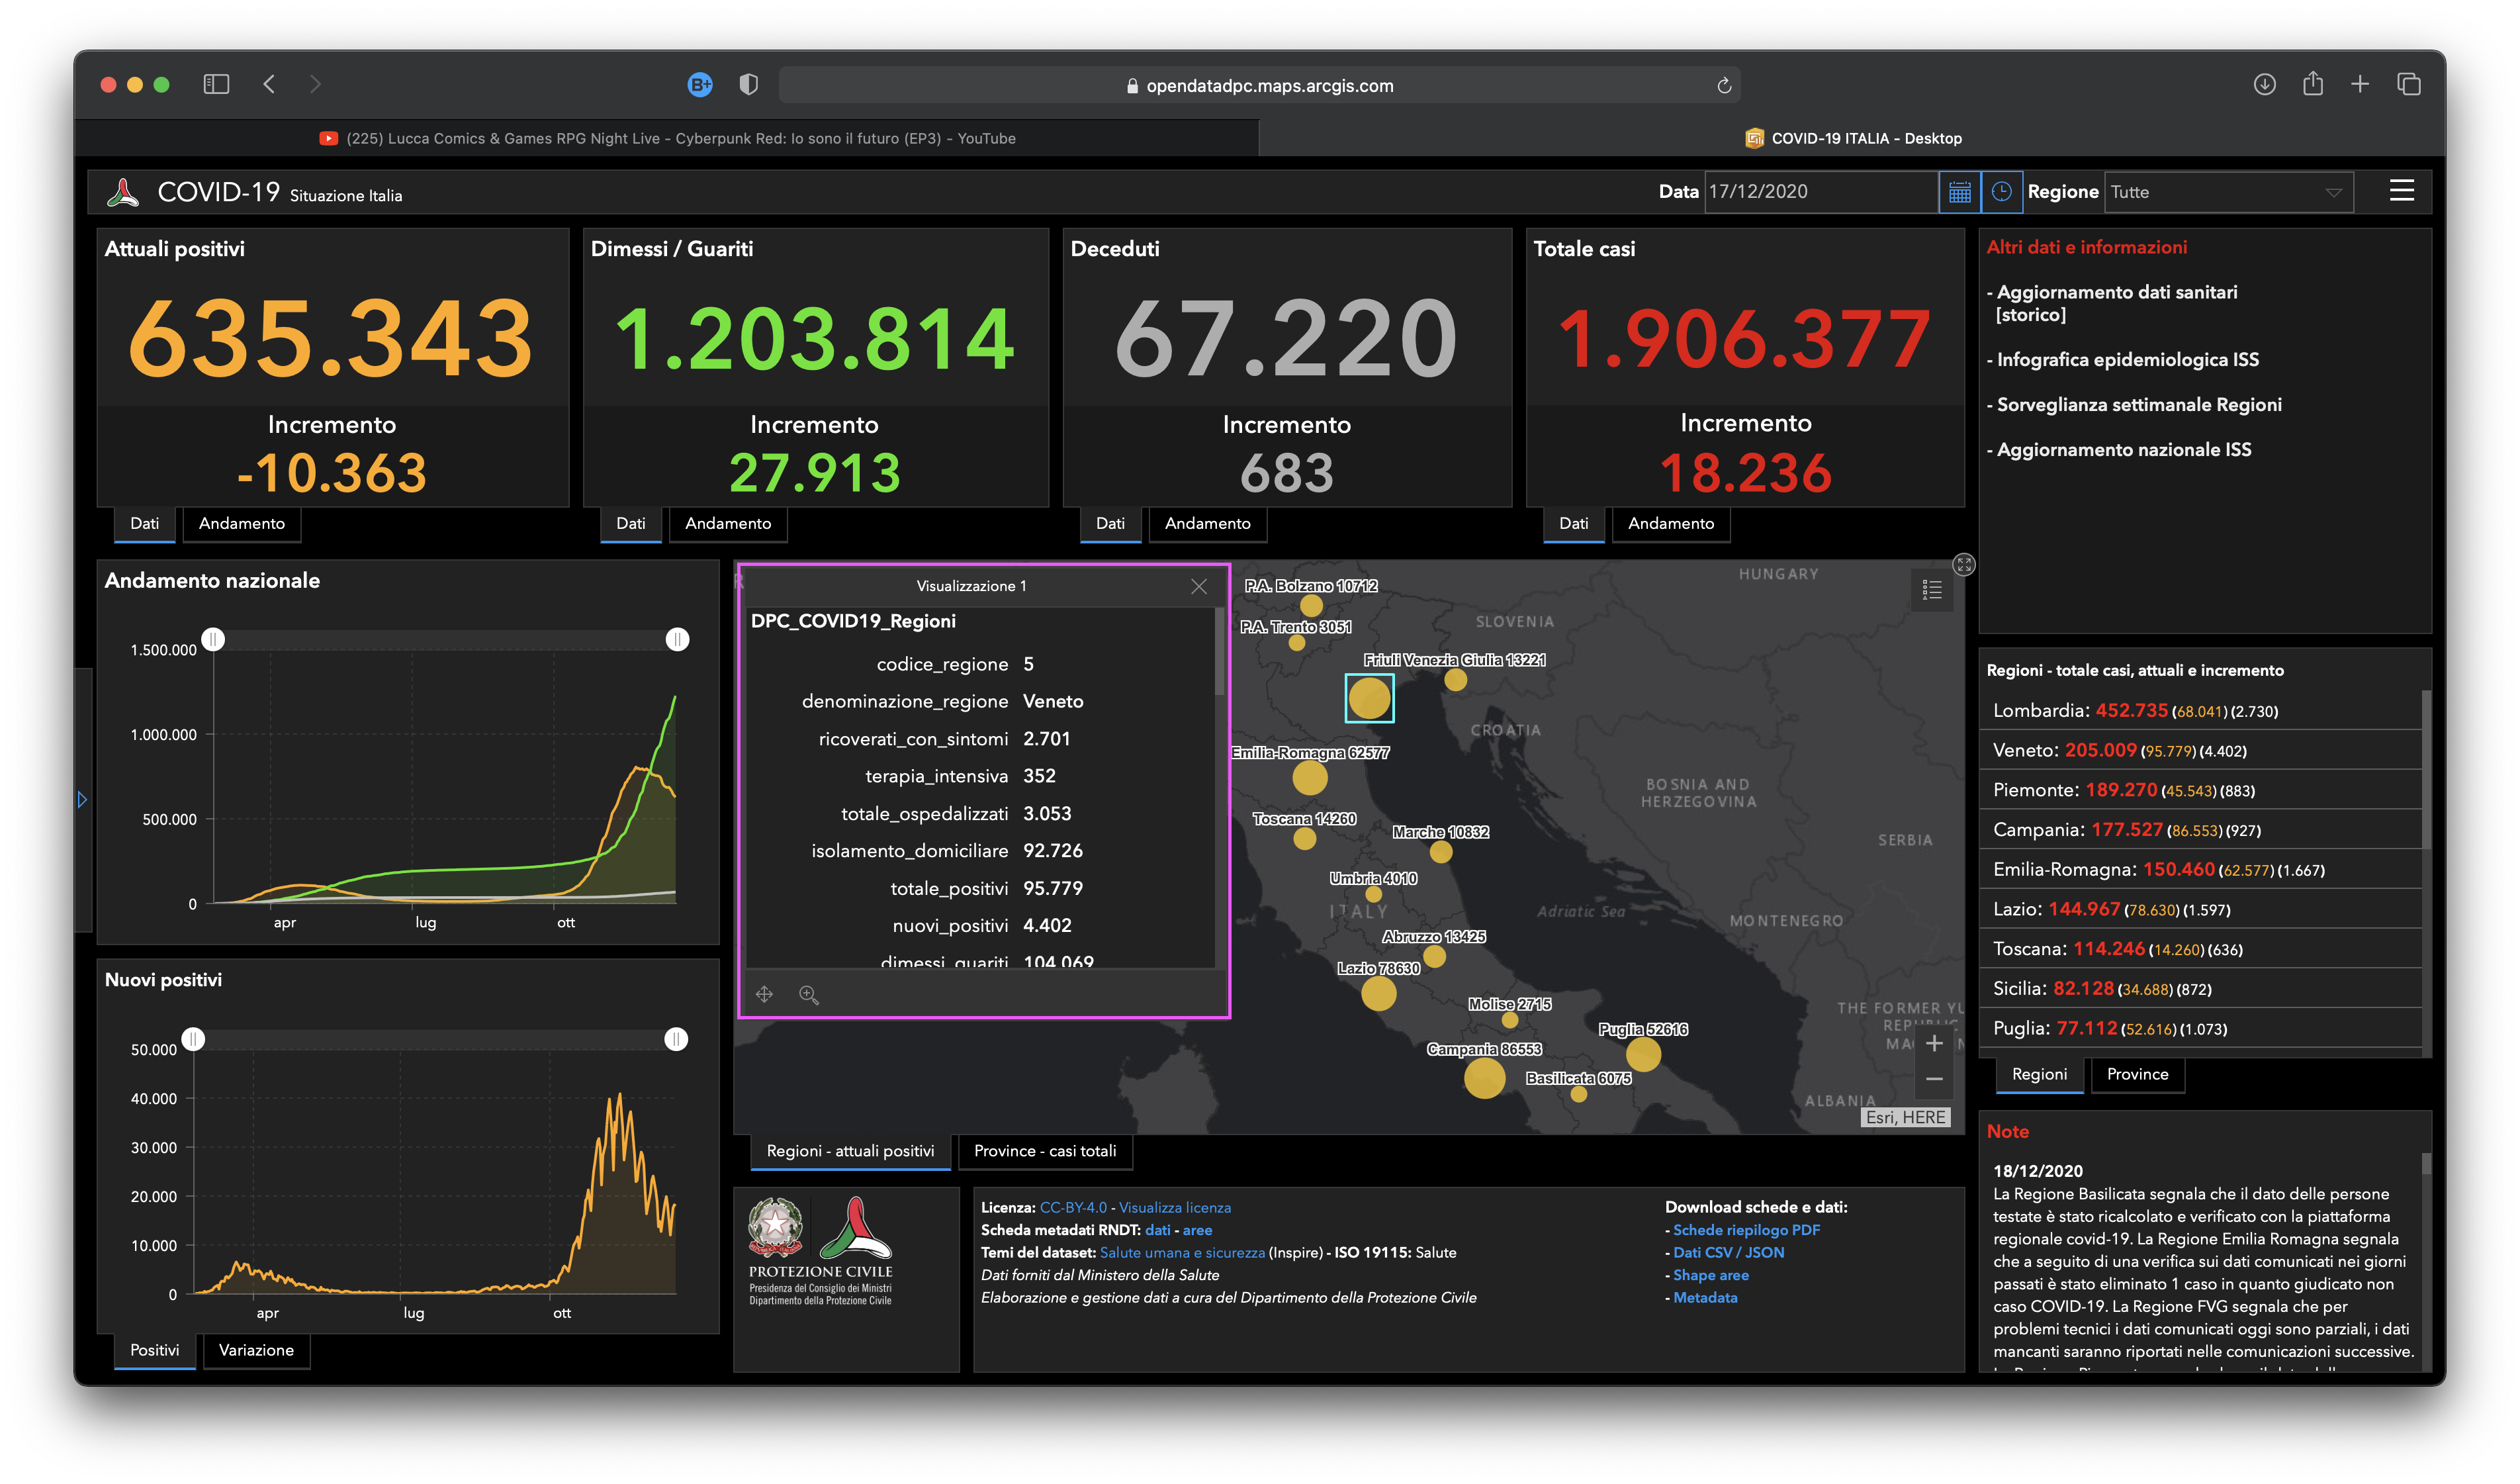
\includegraphics[width=\columnwidth]{../../../assets/images/verifica-risorse-esistenti/guidelines_violations_10}
                \caption{Dettaglio di quando si clicca sul pallino giallo di una regione sulla mappa.}
            \end{subfigure}
            
            \begin{subfigure}[b]{0.5\columnwidth}
                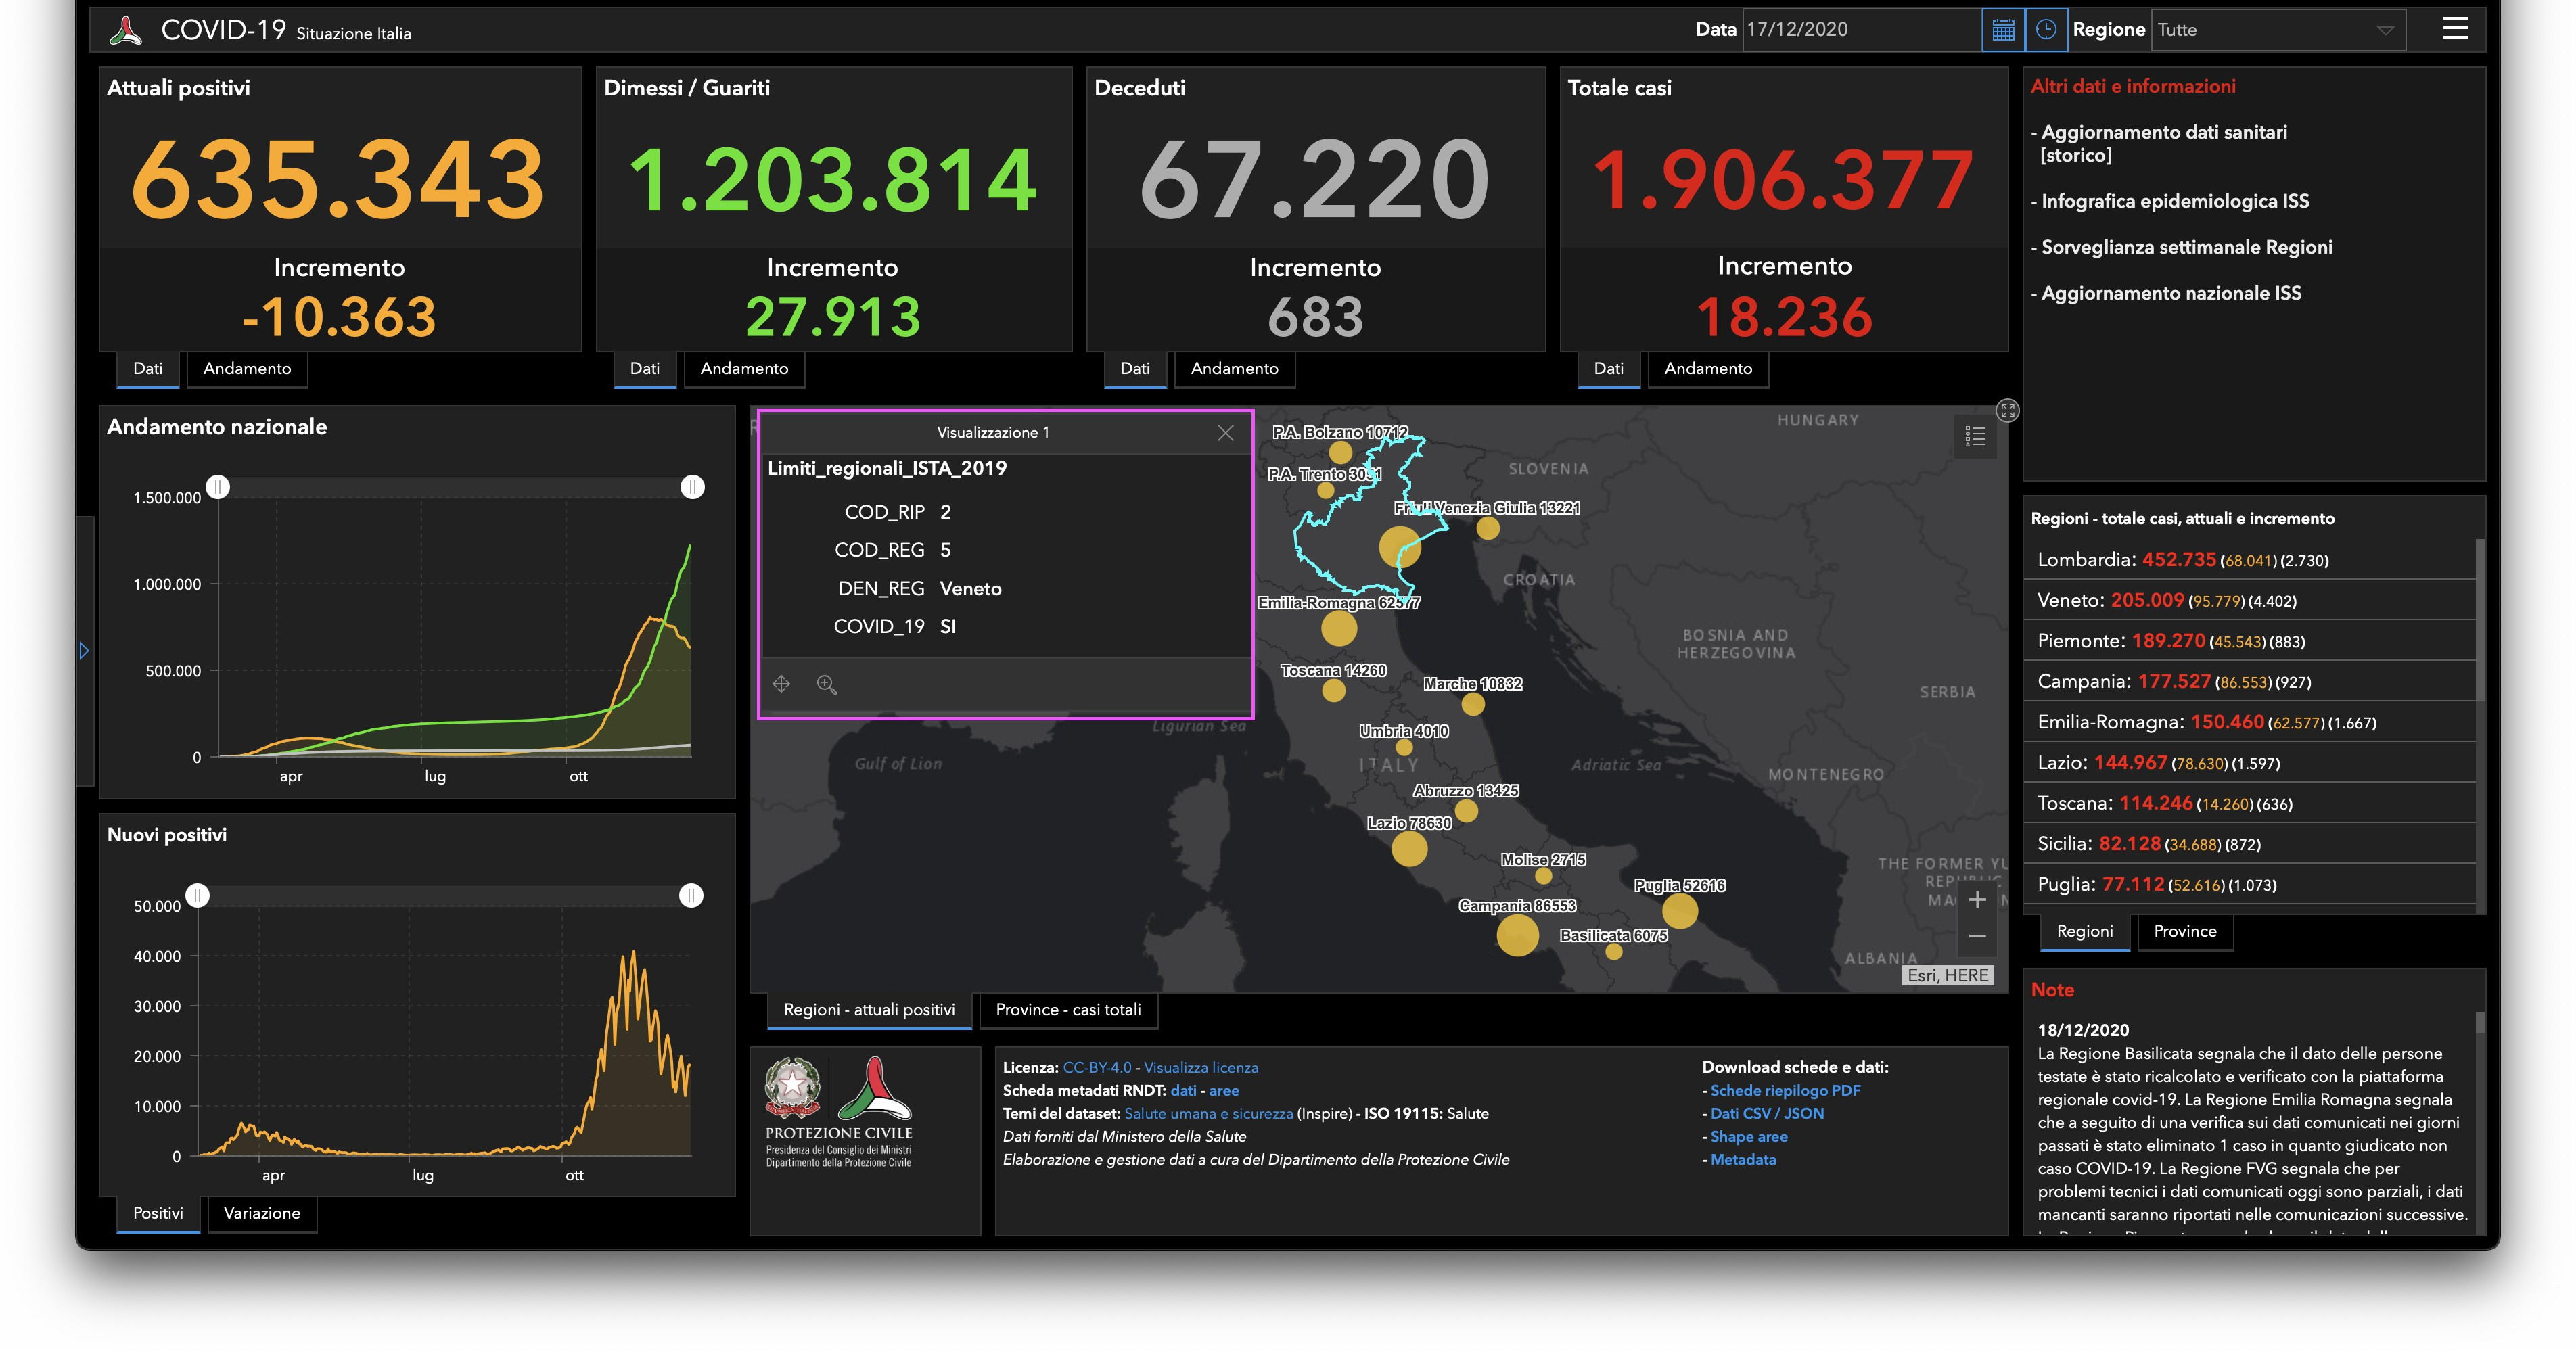
\includegraphics[width=\columnwidth]{../../../assets/images/verifica-risorse-esistenti/guidelines_violations_11}
                \caption{Dettaglio di quando si clicca sull'area di una regione sulla mappa.}
            \end{subfigure}

            \begin{subfigure}[b]{0.5\columnwidth}
                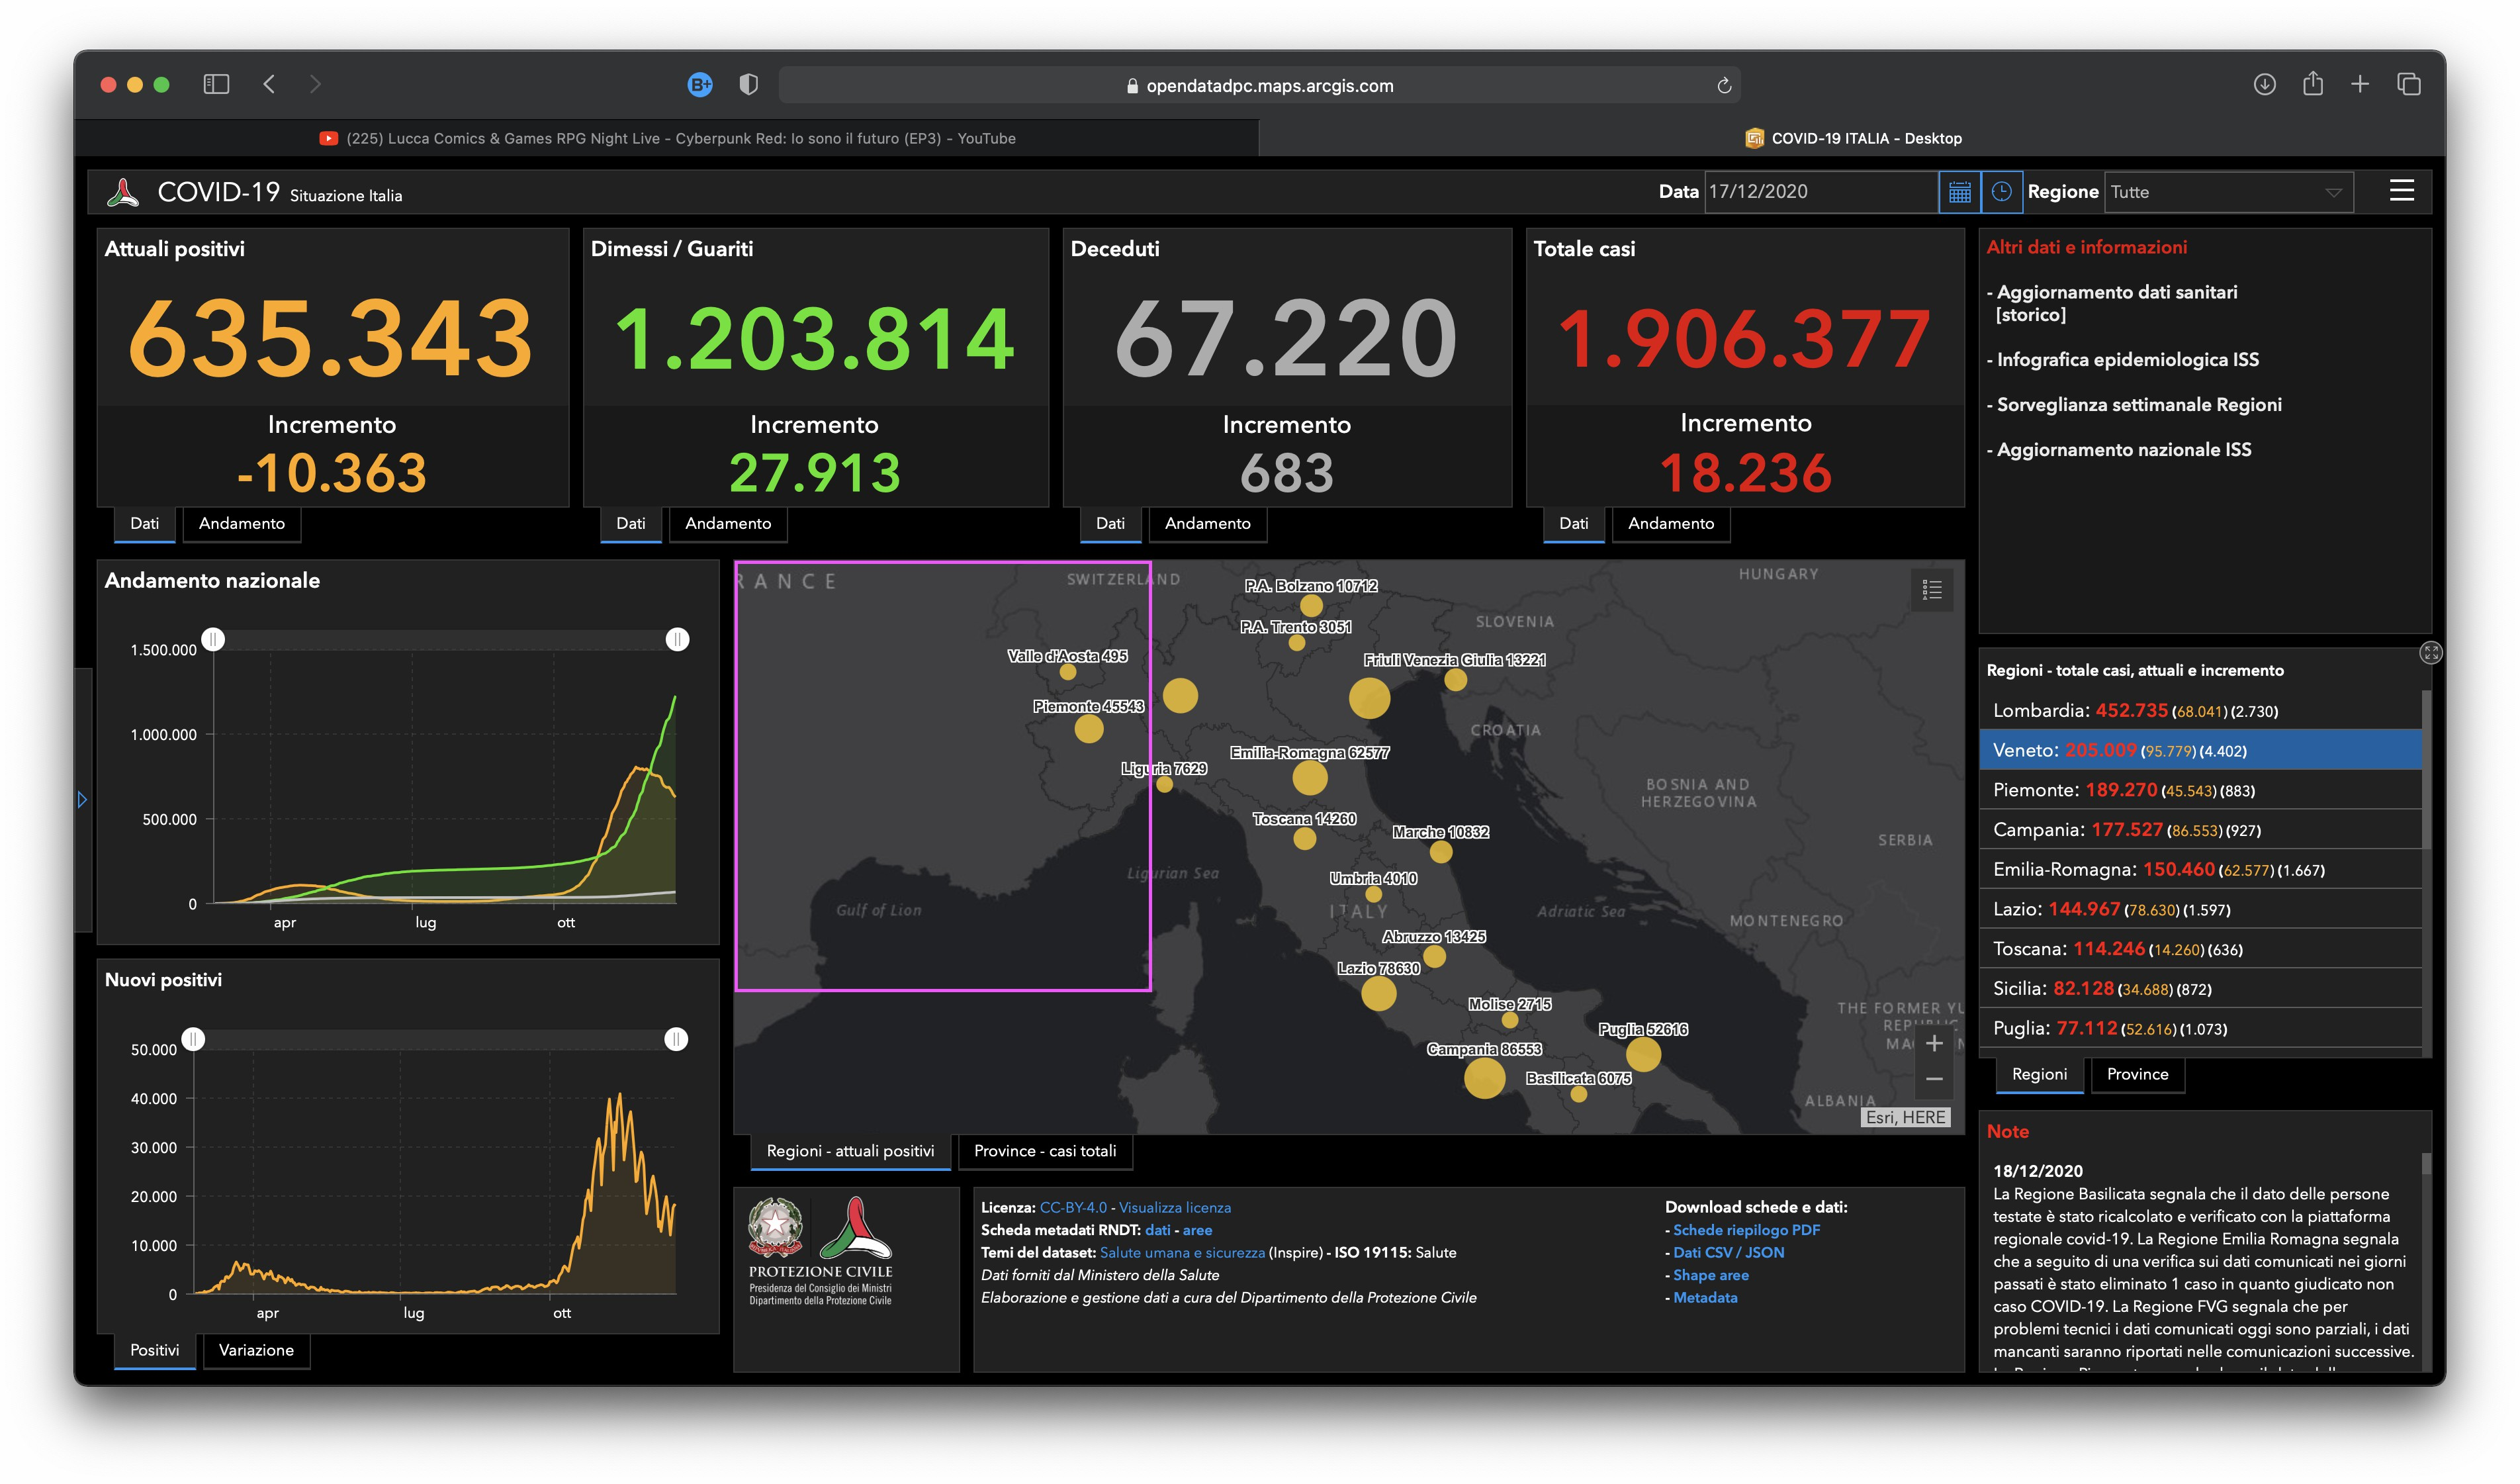
\includegraphics[width=\columnwidth]{../../../assets/images/verifica-risorse-esistenti/guidelines_violations_12}
                \caption{Dettaglio di quando si clicca su di una regione nella lista a destra.}
            \end{subfigure}

            \caption{Violazione della linea guida 29: non predicibilità dei comportamenti.}
            \label{fig:guidelines-violations-10}
        \end{figure}
    \item Rispettata;
    \item I testi, evidenziati, in ~\ref{fig:guidelines-violations-11} hanno la dimensioni del font eccessivamente piccola seppur ci sia abbastanza spazio per ingrandirla;
        \begin{figure}[H]
            \centering
            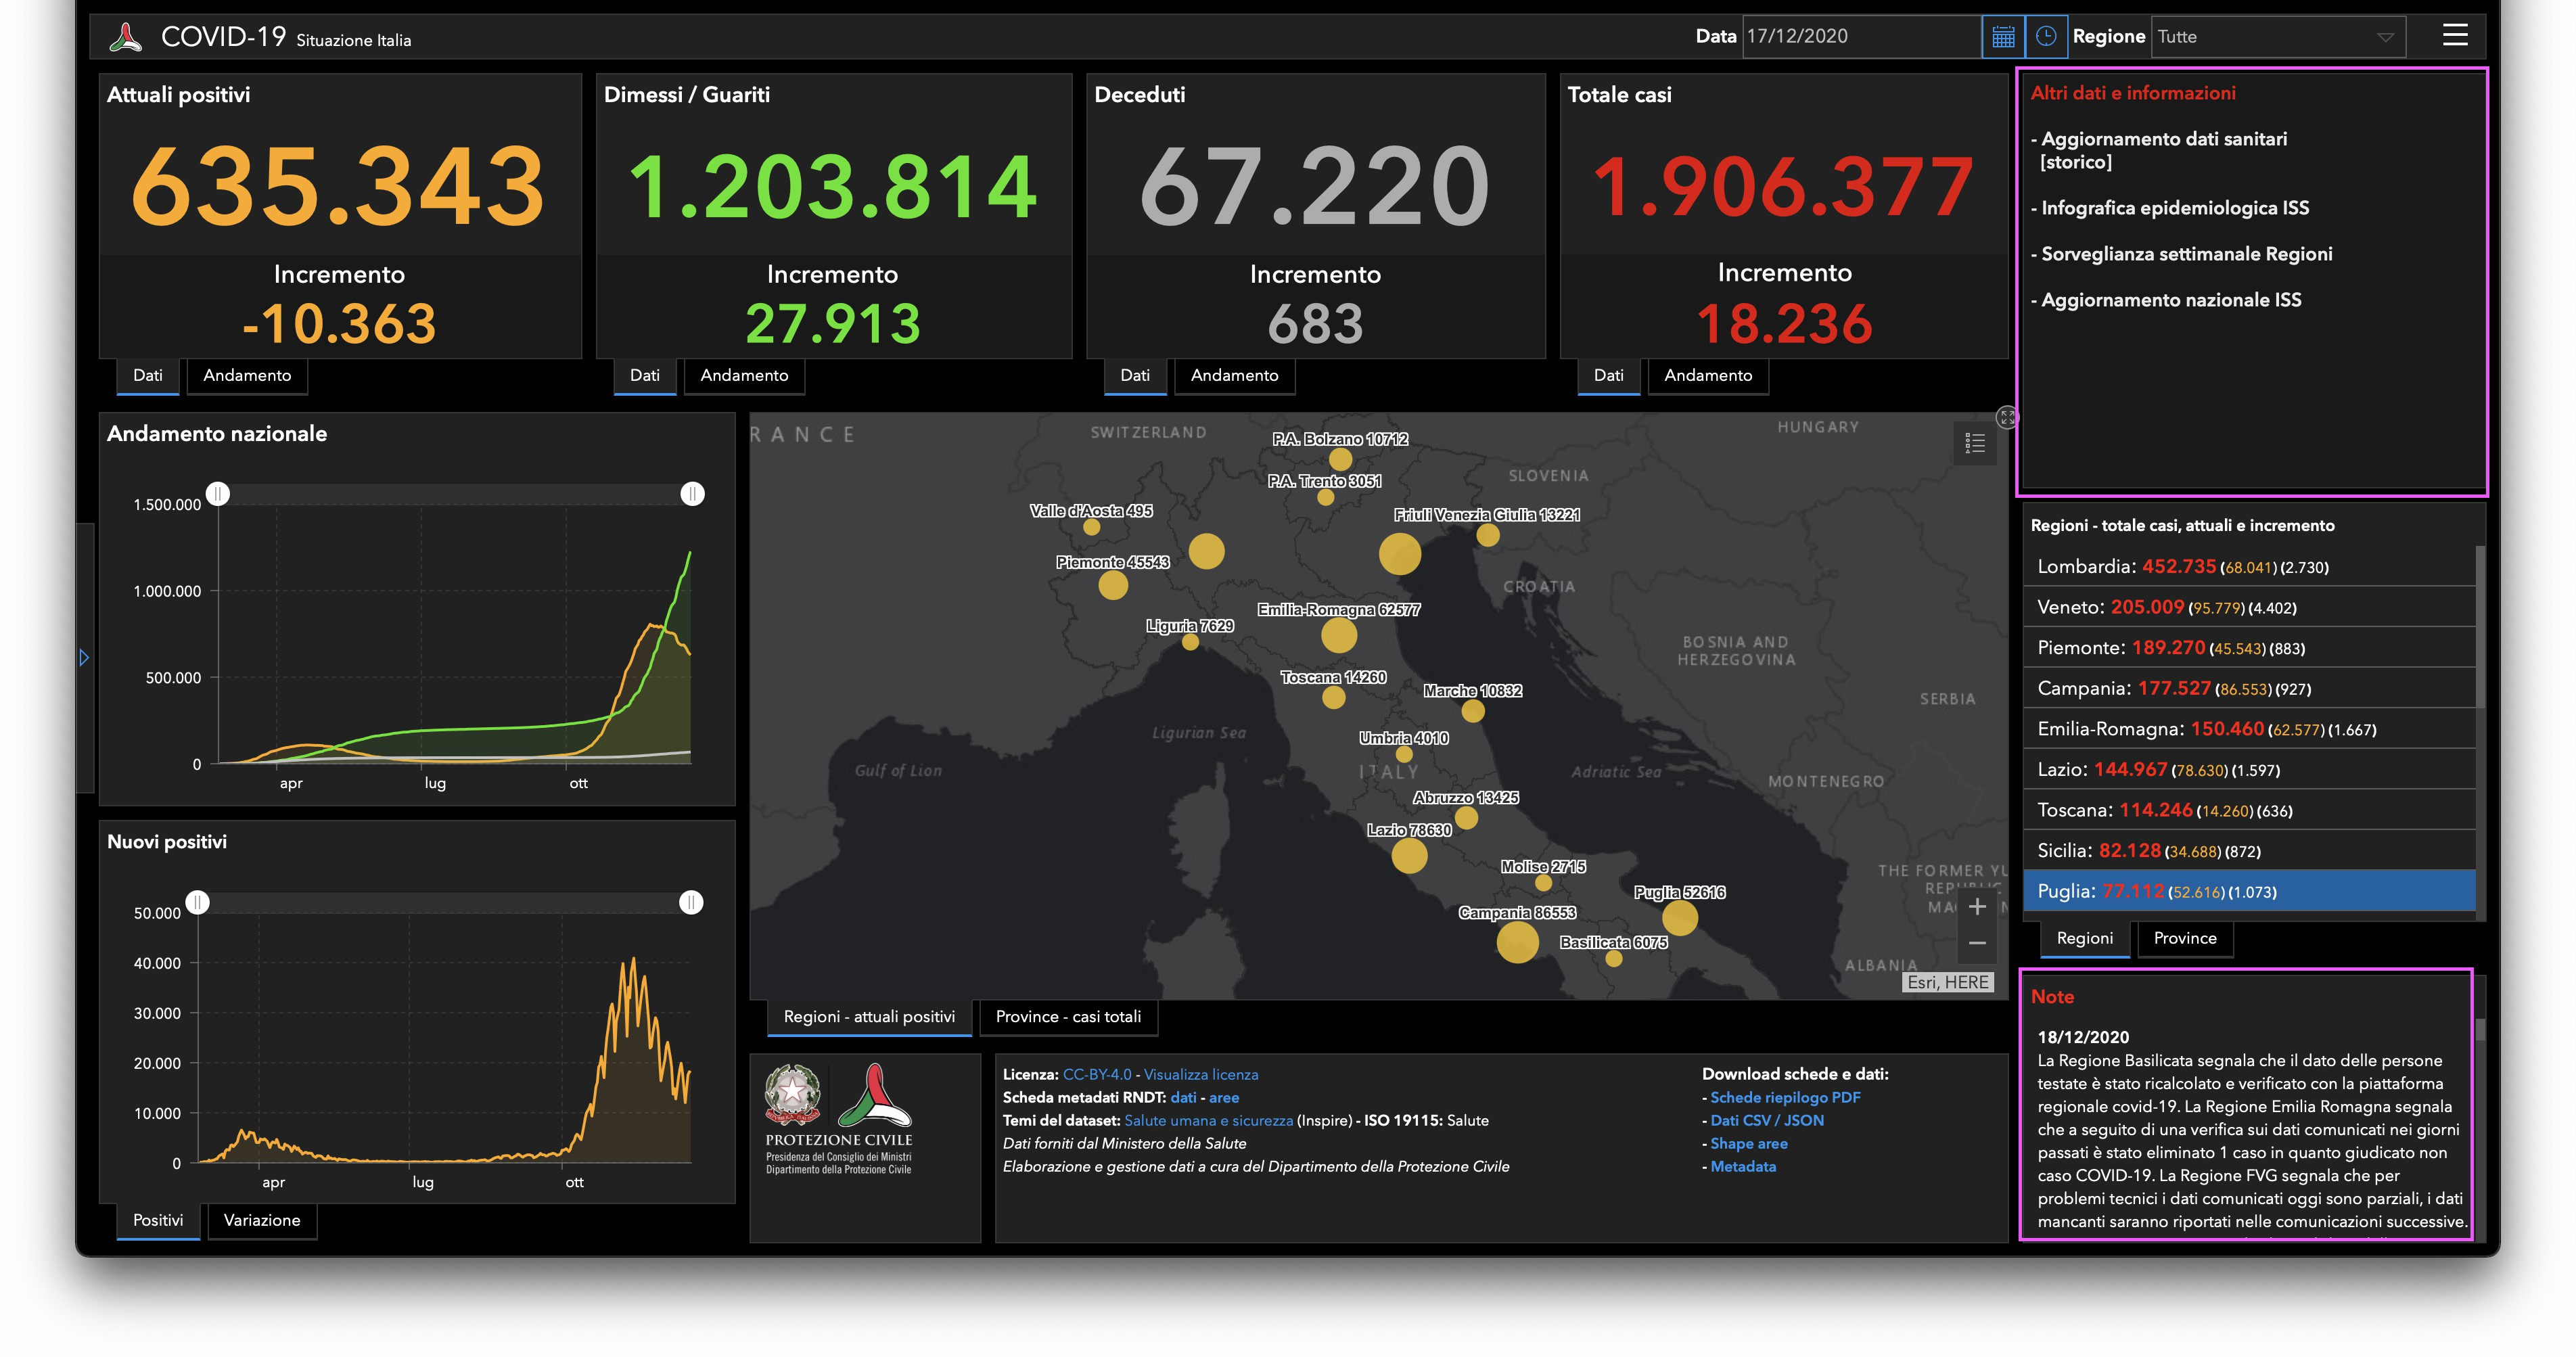
\includegraphics[width=0.5\columnwidth]{../../../assets/images/verifica-risorse-esistenti/guidelines_violations_13}
            \caption{Violazione della linea guida 31: i testi sono molto piccoli e la densità non risulta omogenea.}
            \label{fig:guidelines-violations-11}
        \end{figure}
    \item Le regioni nell'elenco di destra sono cliccabile ma non viene scatenata alcuna azione, confondendo l'utente;
    \item Non è chiaro a cosa serva il pulsante con icona un orologio evidenziato in ~\ref{fig:guidelines-violations-12} dato che l'orario è indifferente, anzi, se si seleziona un ``orario sbagliato" non viene visualizzato alcun tipo di dato;
        \begin{figure}[H]
            \centering
            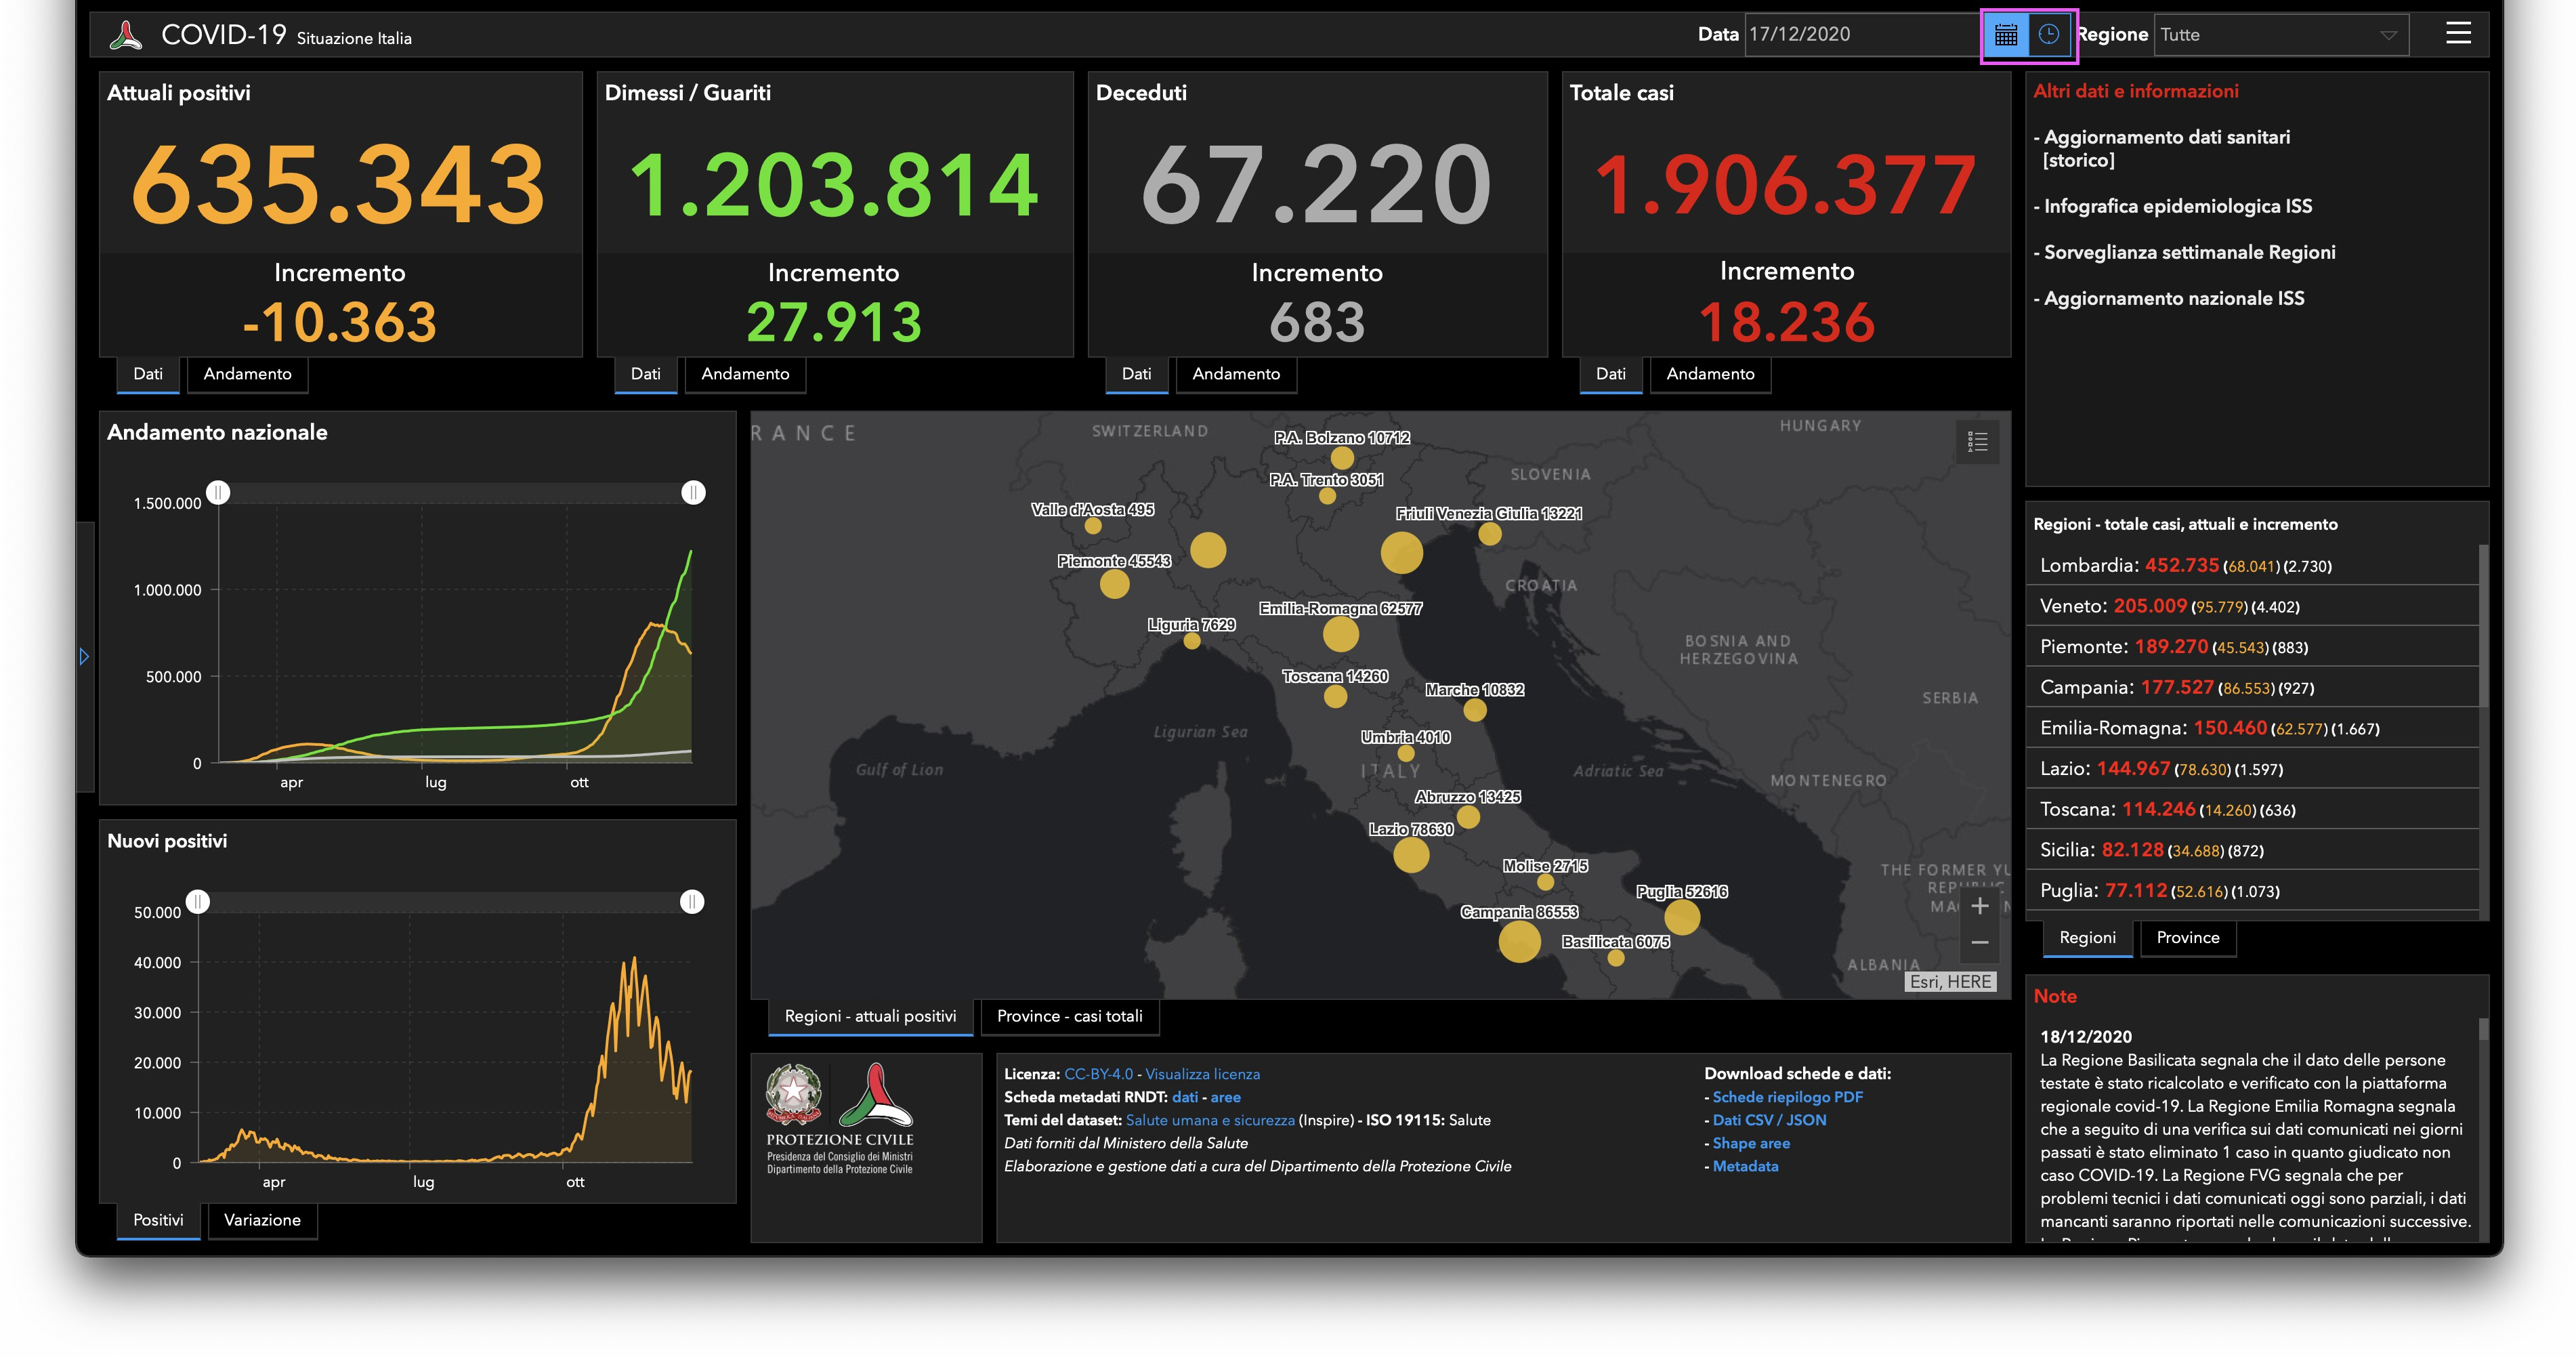
\includegraphics[width=0.5\columnwidth]{../../../assets/images/verifica-risorse-esistenti/guidelines_violations_14}
            \caption{Violazione della linea guida 32: elementi cliccabili che però non compiono alcuna azione.}
            \label{fig:guidelines-violations-12}
        \end{figure}
    \item Rispettata;
    \item I link evidenziati in ~\ref{fig:guidelines-violations-13} non hanno lo stesso stile degli altri link;
        \begin{figure}[H]
            \centering
            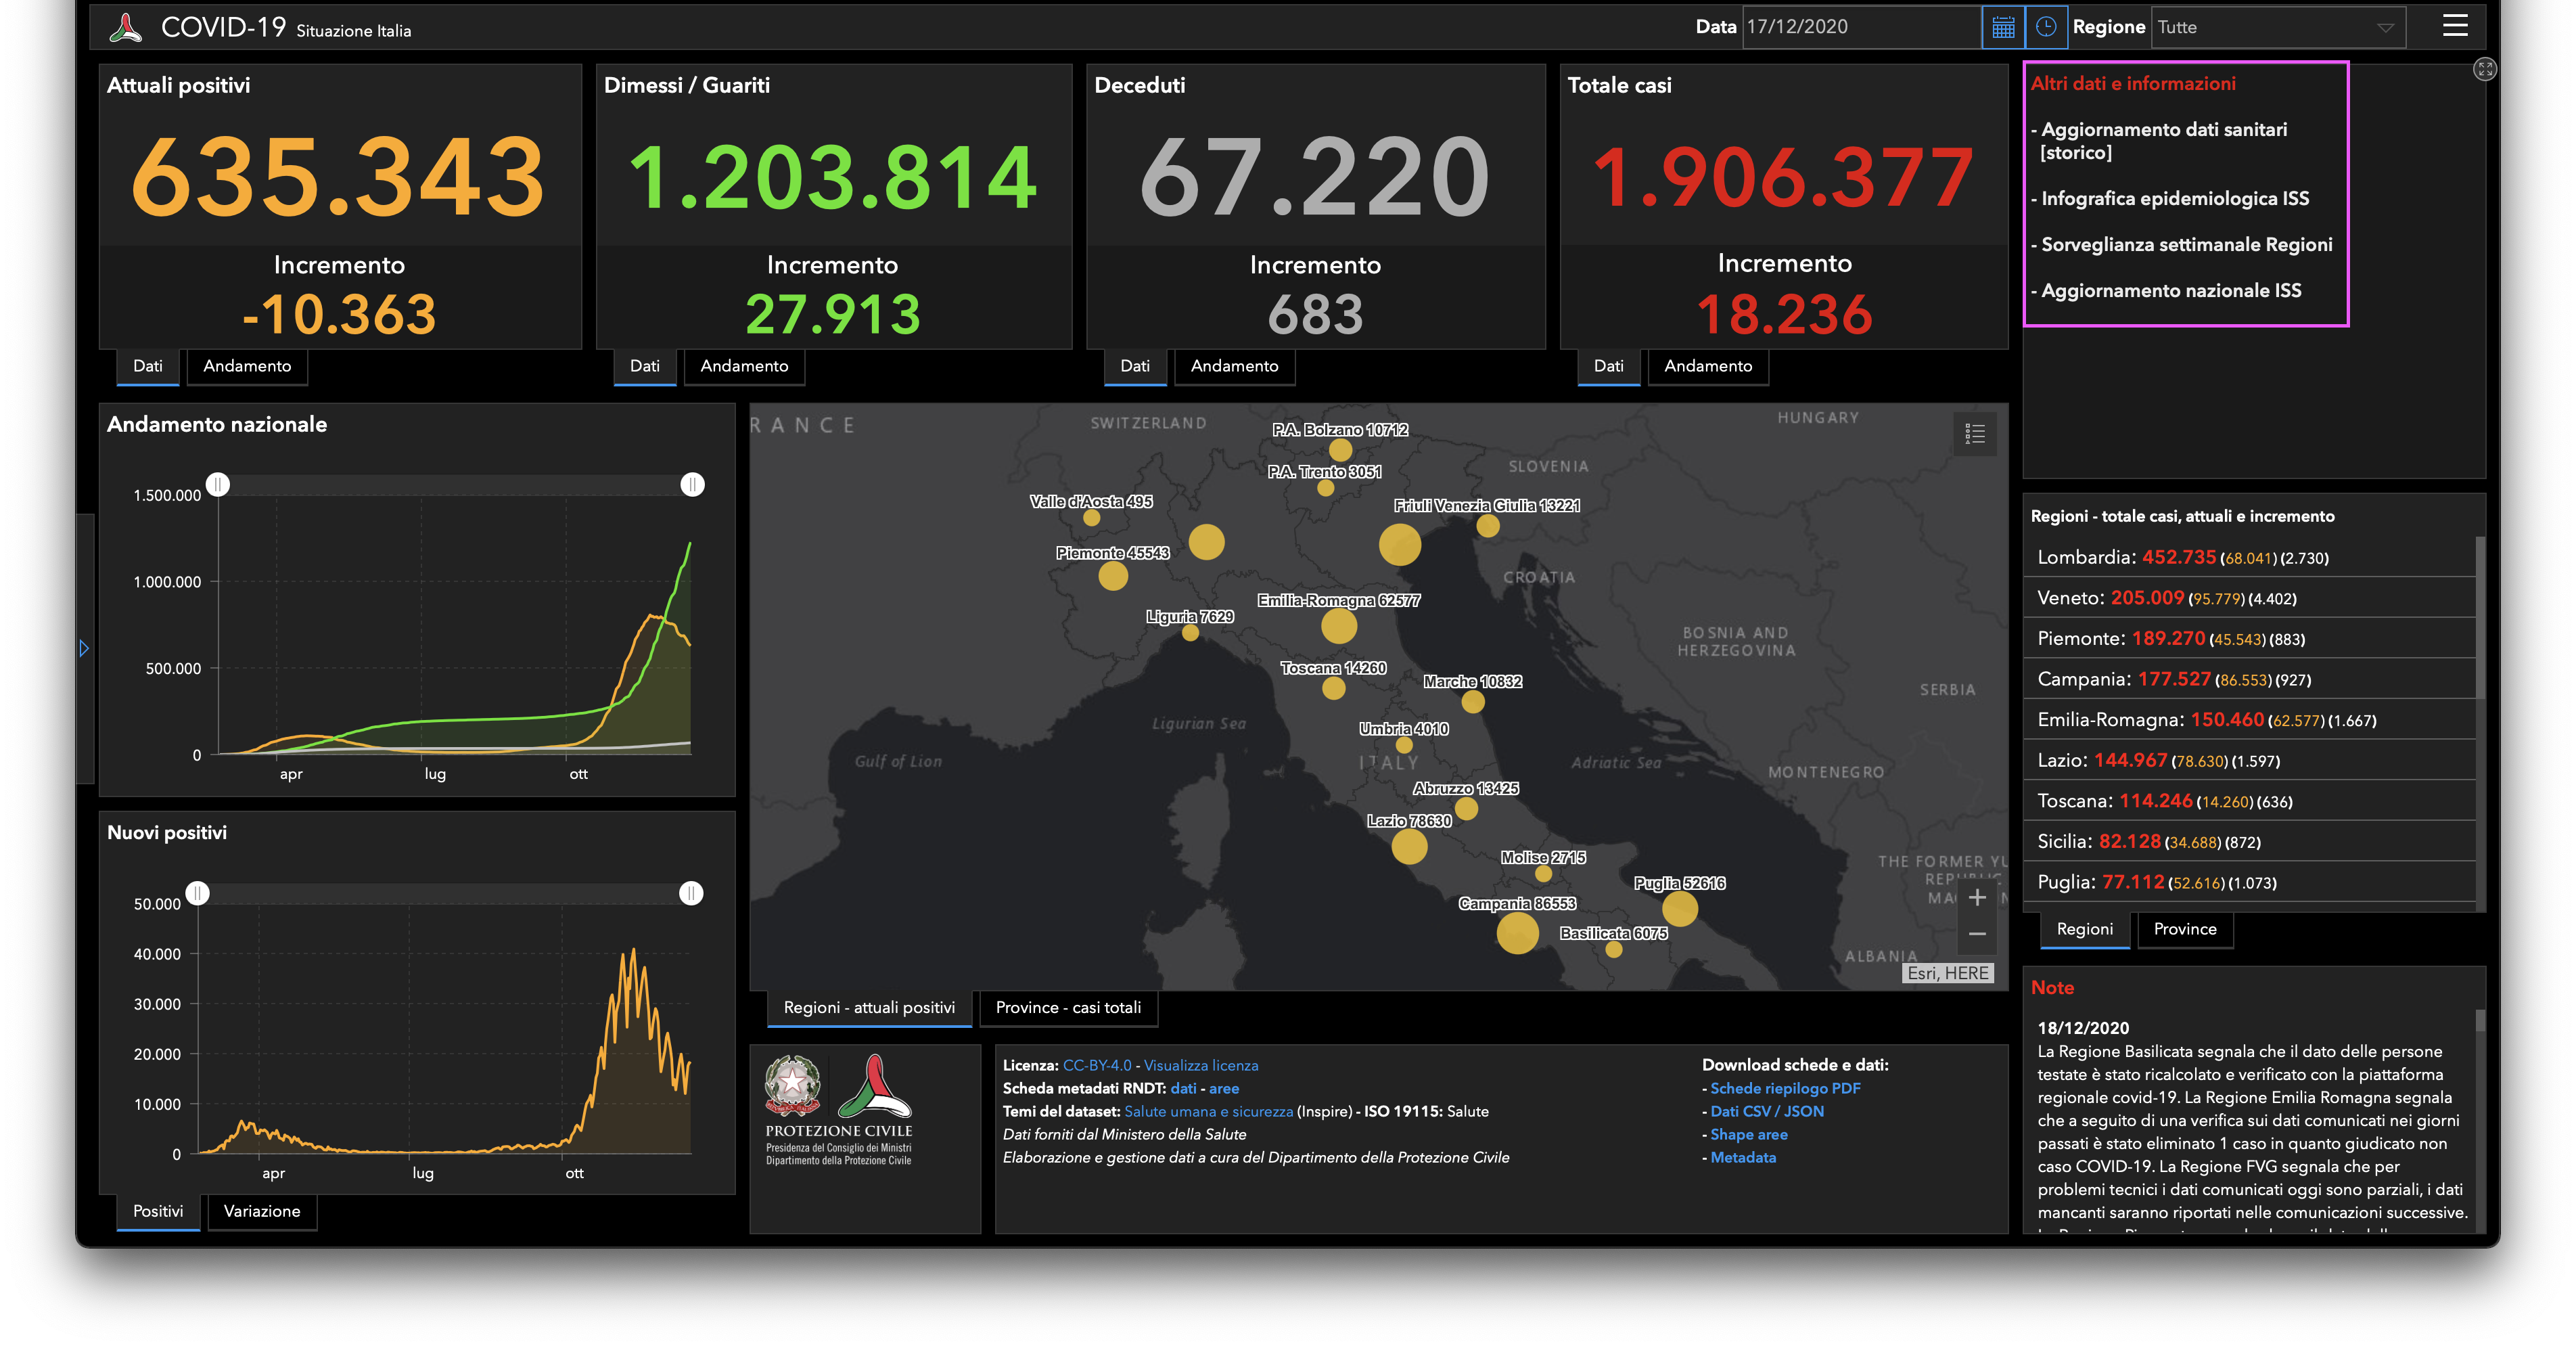
\includegraphics[width=0.5\columnwidth]{../../../assets/images/verifica-risorse-esistenti/guidelines_violations_15}
            \caption{Violazione linea guida 35: i link non hanno tutti lo stesso aspetto.}
            \label{fig:guidelines-violations-13}
        \end{figure}
    \item Non sono presenti legende per i grafici a meno che non ci si passi sopra con il mouse;
    \item Rispettata;
    \item Non è disponibile una versione per la stampa. In ~\ref{fig:guidelines-violations-14} abbiamo provato a stampare la pagina della dashboard;
        \begin{figure}[H]
            \centering
            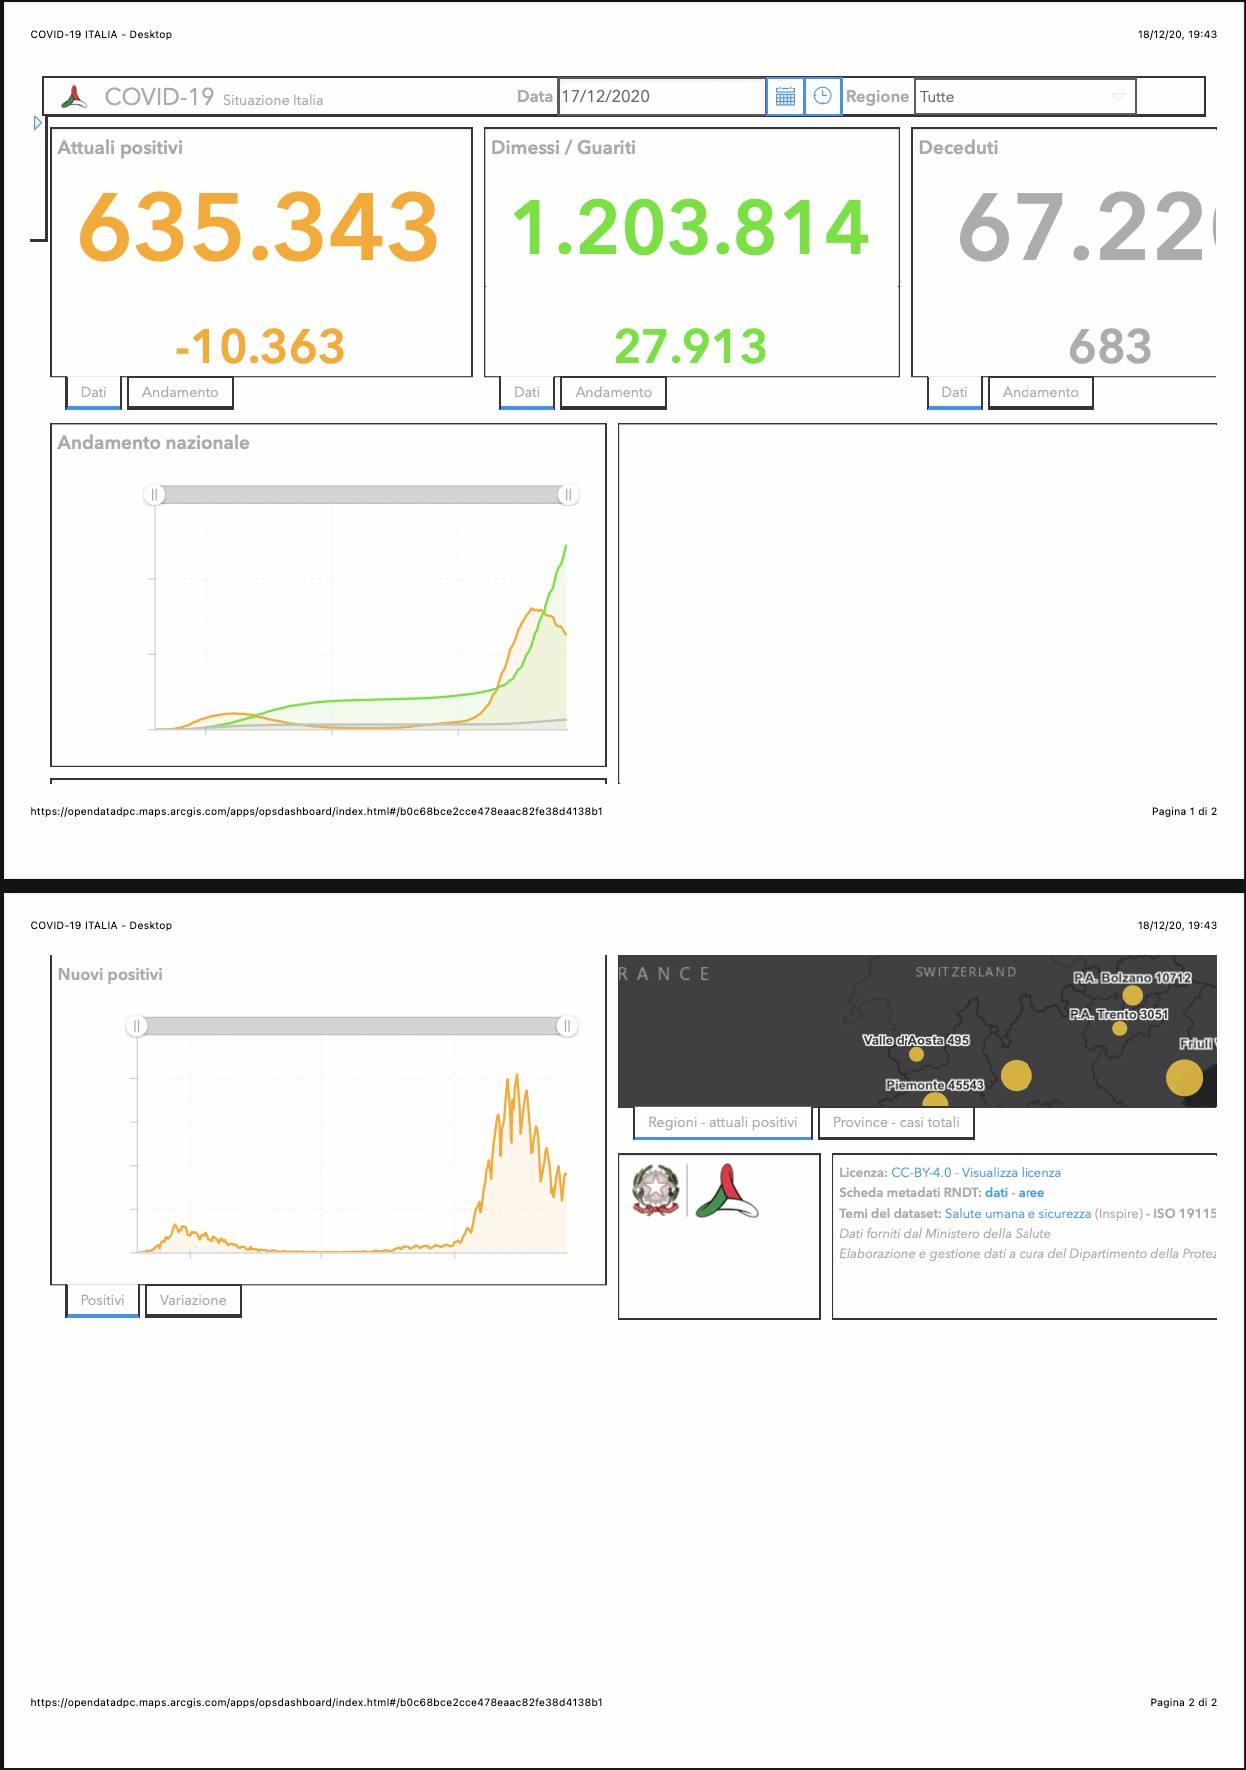
\includegraphics[width=0.5\columnwidth]{../../../assets/images/verifica-risorse-esistenti/guidelines_violations_16}
            \caption{Violazione della linea guida 38: non è disponibile una versione per la stampa.}
            \label{fig:guidelines-violations-14}
        \end{figure}
    \item Rispettata;
    \item Rispettata;
    \item La disposizione in griglie, come si può notare in  ~\ref{fig:guidelines-violations-15}, non sono rispettate;
        \begin{figure}[H]
            \centering
            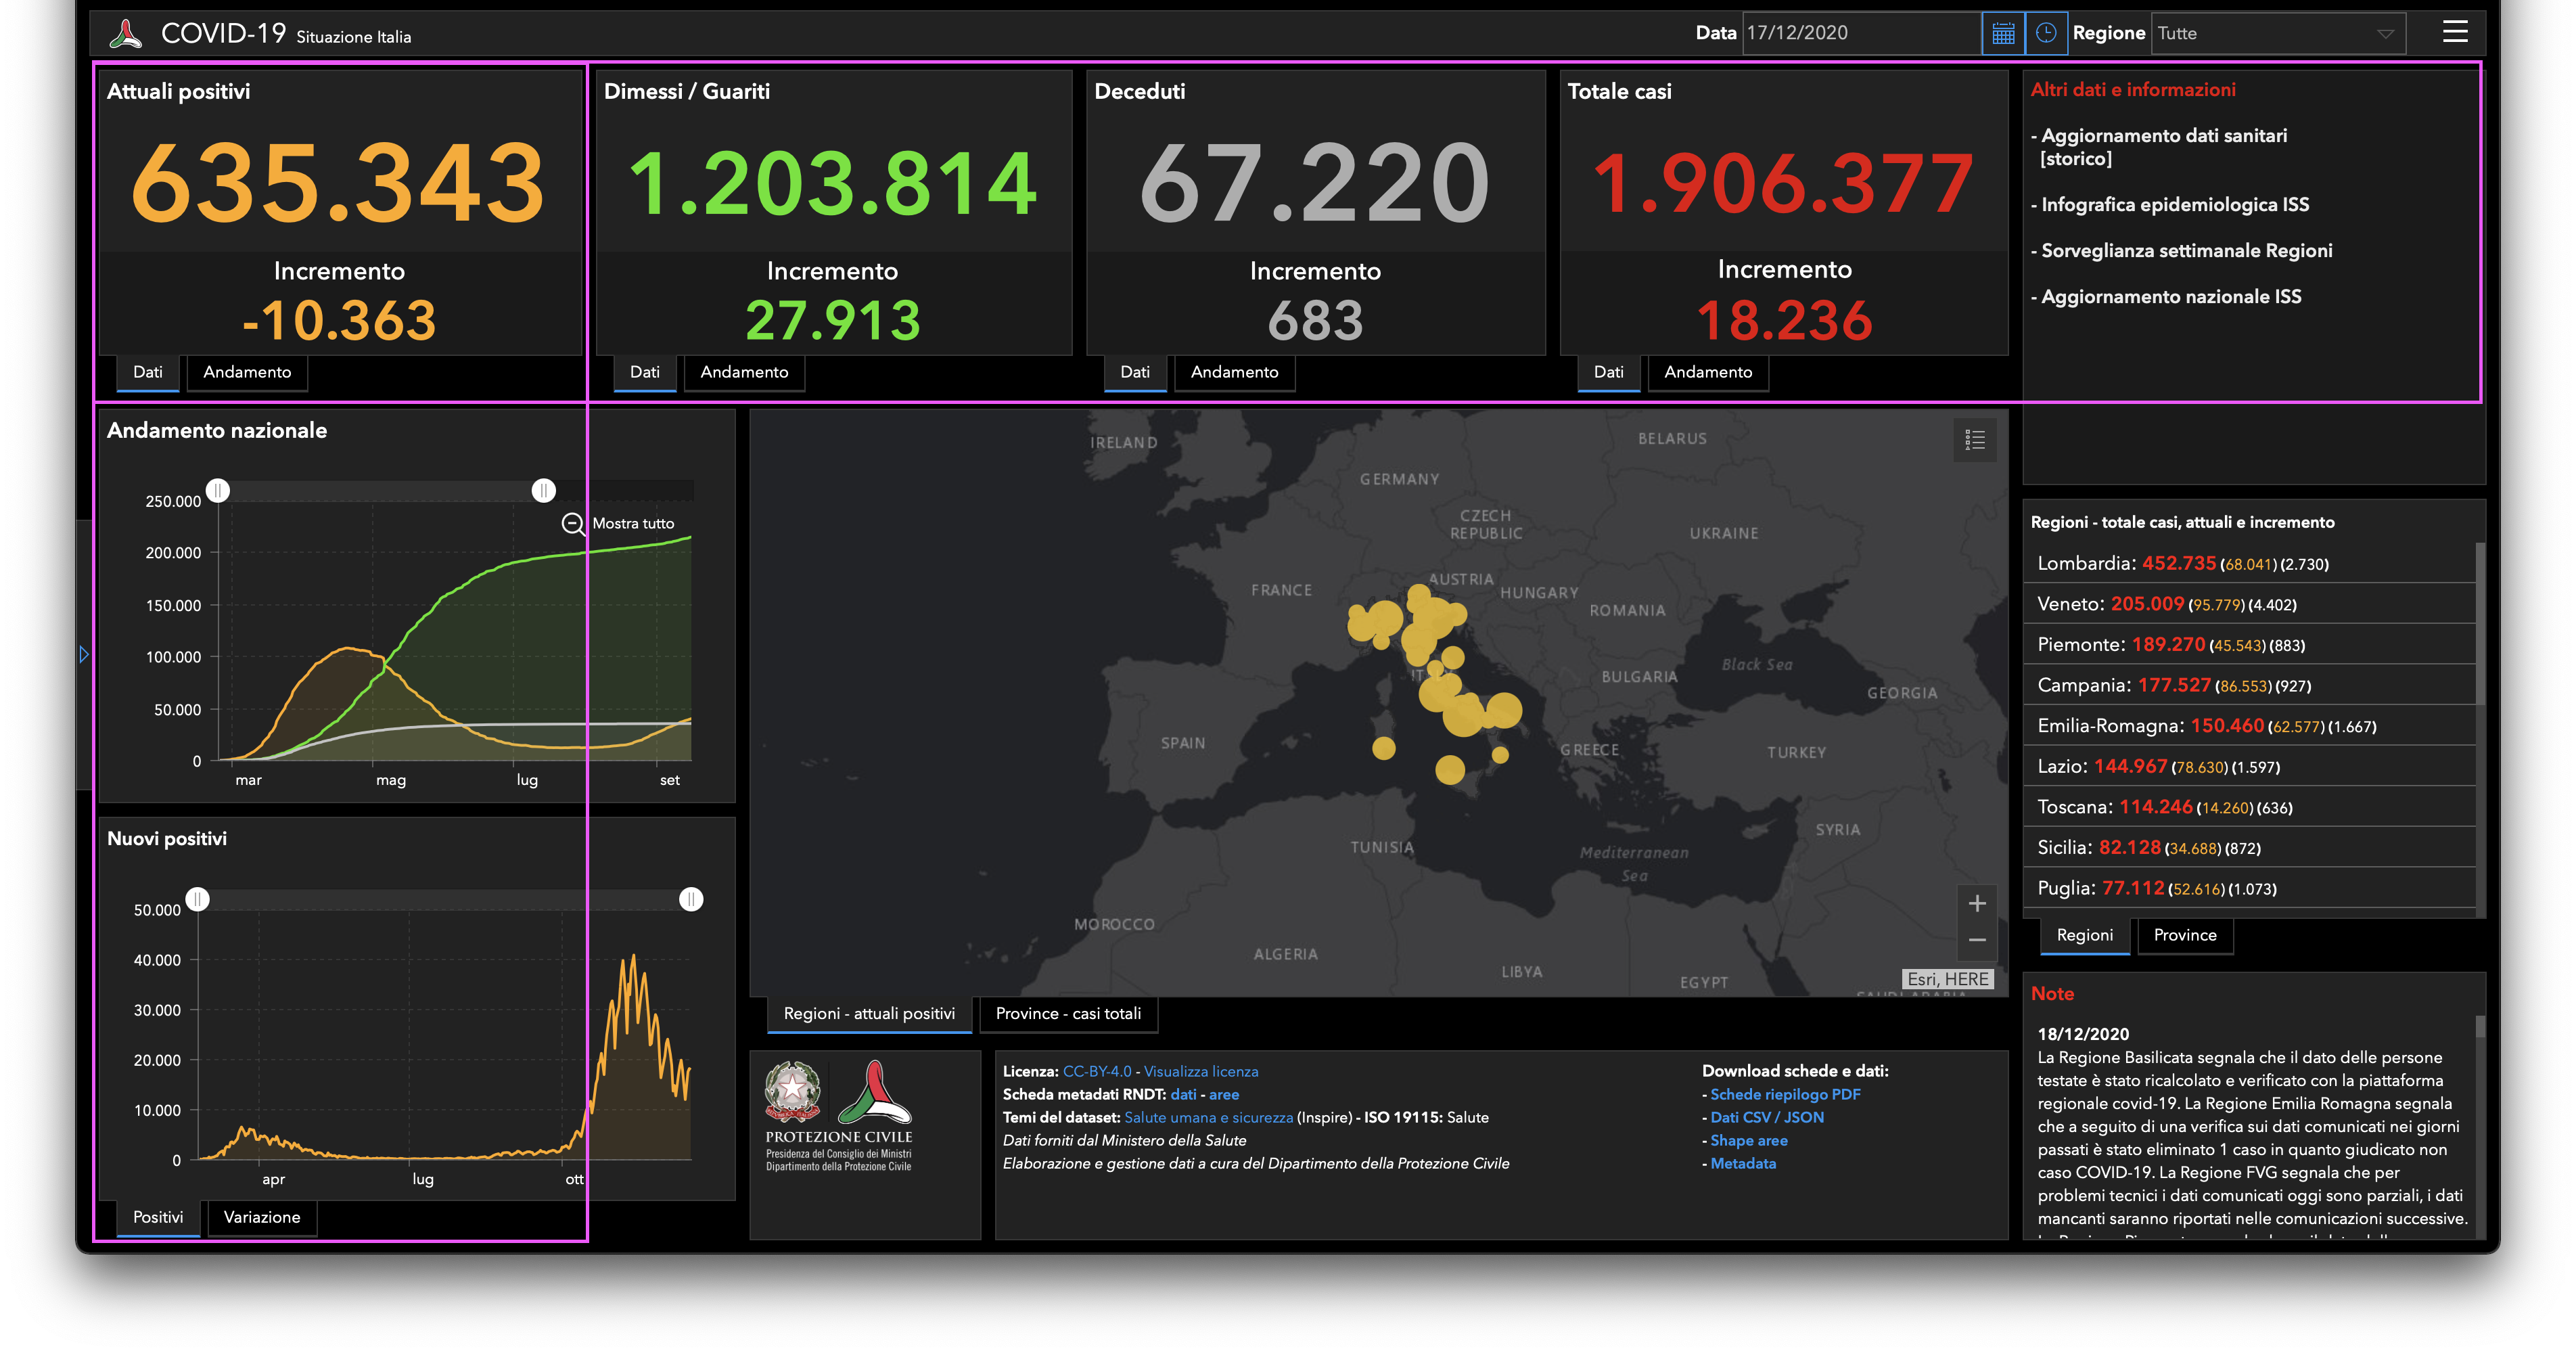
\includegraphics[width=0.5\columnwidth]{../../../assets/images/verifica-risorse-esistenti/guidelines_violations_17}
            \caption{Violazione della linea guida 41: la disposizione in griglie non è rispettata.}
            \label{fig:guidelines-violations-15}
        \end{figure}
    \item Rispettata.
\end{enumerate}
